% Options for packages loaded elsewhere
\PassOptionsToPackage{unicode}{hyperref}
\PassOptionsToPackage{hyphens}{url}
\PassOptionsToPackage{dvipsnames,svgnames*,x11names*}{xcolor}
%
\documentclass[
  11pt,
]{article}
\usepackage[]{mathpazo}
\usepackage{amsmath}
\usepackage{ifxetex,ifluatex}
\ifnum 0\ifxetex 1\fi\ifluatex 1\fi=0 % if pdftex
  \usepackage[T1]{fontenc}
  \usepackage[utf8]{inputenc}
  \usepackage{textcomp} % provide euro and other symbols
  \usepackage{amssymb}
\else % if luatex or xetex
  \usepackage{unicode-math}
  \defaultfontfeatures{Scale=MatchLowercase}
  \defaultfontfeatures[\rmfamily]{Ligatures=TeX,Scale=1}
\fi
% Use upquote if available, for straight quotes in verbatim environments
\IfFileExists{upquote.sty}{\usepackage{upquote}}{}
\IfFileExists{microtype.sty}{% use microtype if available
  \usepackage[]{microtype}
  \UseMicrotypeSet[protrusion]{basicmath} % disable protrusion for tt fonts
}{}
\usepackage{xcolor}
\IfFileExists{xurl.sty}{\usepackage{xurl}}{} % add URL line breaks if available
\IfFileExists{bookmark.sty}{\usepackage{bookmark}}{\usepackage{hyperref}}
\hypersetup{
  pdftitle={Making Migration Sexy: How State and National Policies Influence Migration of Same-Sex Couples},
  pdfauthor={Nathan I. Hoffmann, Department of Sociology, University of California, Los Angeles; Kristopher Velasco, Department of Sociology, University of Texas at Austin},
  pdfkeywords={immigration, same-sex couples, LGBTQ policy, sexuality},
  colorlinks=true,
  linkcolor=blue,
  filecolor=Maroon,
  citecolor=Blue,
  urlcolor=Blue,
  pdfcreator={LaTeX via pandoc}}
\urlstyle{same} % disable monospaced font for URLs
\usepackage[margin=1in]{geometry}
\usepackage{longtable,booktabs}
\usepackage{calc} % for calculating minipage widths
% Correct order of tables after \paragraph or \subparagraph
\usepackage{etoolbox}
\makeatletter
\patchcmd\longtable{\par}{\if@noskipsec\mbox{}\fi\par}{}{}
\makeatother
% Allow footnotes in longtable head/foot
\IfFileExists{footnotehyper.sty}{\usepackage{footnotehyper}}{\usepackage{footnote}}
\makesavenoteenv{longtable}
\usepackage{graphicx}
\makeatletter
\def\maxwidth{\ifdim\Gin@nat@width>\linewidth\linewidth\else\Gin@nat@width\fi}
\def\maxheight{\ifdim\Gin@nat@height>\textheight\textheight\else\Gin@nat@height\fi}
\makeatother
% Scale images if necessary, so that they will not overflow the page
% margins by default, and it is still possible to overwrite the defaults
% using explicit options in \includegraphics[width, height, ...]{}
\setkeys{Gin}{width=\maxwidth,height=\maxheight,keepaspectratio}
% Set default figure placement to htbp
\makeatletter
\def\fps@figure{htbp}
\makeatother
\setlength{\emergencystretch}{3em} % prevent overfull lines
\providecommand{\tightlist}{%
  \setlength{\itemsep}{0pt}\setlength{\parskip}{0pt}}
\setcounter{secnumdepth}{-\maxdimen} % remove section numbering
\usepackage{fancyhdr}
\pagestyle{fancy}
\setlength{\headheight}{13.6pt}
\rhead{\textit{Hoffmann and Velasco}}
\usepackage{booktabs}
\usepackage{longtable}
\usepackage{array}
\usepackage{multirow}
\usepackage{wrapfig}
\usepackage{float}
\usepackage{colortbl}
\usepackage{pdflscape}
\usepackage{tabu}
\usepackage{threeparttable}
\usepackage{threeparttablex}
\usepackage[normalem]{ulem}
\usepackage{makecell}
\usepackage{xcolor}
\ifluatex
  \usepackage{selnolig}  % disable illegal ligatures
\fi
\newlength{\cslhangindent}
\setlength{\cslhangindent}{1.5em}
\newlength{\csllabelwidth}
\setlength{\csllabelwidth}{3em}
\newenvironment{CSLReferences}[2] % #1 hanging-ident, #2 entry spacing
 {% don't indent paragraphs
  \setlength{\parindent}{0pt}
  % turn on hanging indent if param 1 is 1
  \ifodd #1 \everypar{\setlength{\hangindent}{\cslhangindent}}\ignorespaces\fi
  % set entry spacing
  \ifnum #2 > 0
  \setlength{\parskip}{#2\baselineskip}
  \fi
 }%
 {}
\usepackage{calc}
\newcommand{\CSLBlock}[1]{#1\hfill\break}
\newcommand{\CSLLeftMargin}[1]{\parbox[t]{\csllabelwidth}{#1}}
\newcommand{\CSLRightInline}[1]{\parbox[t]{\linewidth - \csllabelwidth}{#1}\break}
\newcommand{\CSLIndent}[1]{\hspace{\cslhangindent}#1}

\title{Making Migration Sexy: How State and National Policies Influence Migration of Same-Sex Couples\thanks{The authors contributed equally to this project.}}
\author{Nathan I. Hoffmann, Department of Sociology, University of California, Los Angeles \and Kristopher Velasco, Department of Sociology, University of Texas at Austin}
\date{April 8, 2021}

\begin{document}
\maketitle
\begin{abstract}
As same-sex couples gain greater social acceptance and new rights, their numbers in the United States are rapidly increasing. Yet few researchers have studied immigrants in same-sex couples on a large scale. Using the American Community Survey from 2008 to 2019, this study compares immigrants in same-sex couples to corresponding different-sex couples in order to characterize and assess the scale of ``sexual migration'' to the U.S. Moreover, we evaluate how the policy environment regarding same-sex couples shapes migratory patterns. We find that, compared to different-sex immigrant couples, immigrants in same-sex couples come from richer, more democratic countries that are less represented in immigrant networks. Fixed effects models show that as origin countries become more LGBT-friendly, we see more LGB immigrants from those countries in the U.S. On the individual level, immigrants in same-sex couples are more likely to live in progressive U.S. states, an effect that increases in strength as migrants come from for more LGBT-friendly countries of origin. Our findings put into question dominant models of migration that emphasize economic and network effects, suggesting the importance of considering sexuality as well as political and lifestyle motivations more broadly.
\end{abstract}

\hypertarget{introduction}{%
\section{Introduction}\label{introduction}}

In 2013, the U.S. Supreme Court made a landmark decision overturning the Defense of Marriage Act. This decision reverberated across society. One important outcome was making immigration by same-sex couples more accessible. While numbers of different-sex couples including immigrants increased by 13 percent from 2013 to 2019 (from 8.4 million to 9.5 million), those of immigrant same-sex couples grew from 61 thousand to 107 thousand in the same period, an increase of 75 percent (\protect\hyperlink{ref-u.s.censusbureau_2020}{U.S. Census Bureau, 2020}). Indeed, this time period represents an important moment in which policies governing same-sex couples, both in the U.S. and internationally, are changing rapidly. Although short reports have described the lesbian, gay, and bisexual (LGB) immigrant population (\protect\hyperlink{ref-gates_2013}{Gates, 2013a}; \protect\hyperlink{ref-goldberg_2021}{Goldberg \& Conron, 2021}), immigration research has not explicitly analyzed how policy changes are influencing the migration patterns of individuals in same-sex couples into and across the U.S. This is partly due to the fact that conventional migration research focuses on largely economic, cost-benefit analyses and has only recently begun to factor in the role of social policies (\protect\hyperlink{ref-fitzgerald_2014}{Fitzgerald et al., 2014}). Moreover, while gender has been recently recognized as an integral part of the migration process (\protect\hyperlink{ref-hondagneu-sotelo_2012}{Hondagneu-Sotelo, 2012}; \protect\hyperlink{ref-lutz_2010}{Lutz, 2010}), sexuality has received relatively scant attention. As \protect\hyperlink{ref-carrillo_2018}{Carrillo} (\protect\hyperlink{ref-carrillo_2018}{2018}) demonstrates, however, sexuality is a salient factor determining immigration decisions. We show that differences between immigrants in same-sex couples and those in different-sex couples cannot be explained solely using classic theories of migration; consequently, not making sexuality an integral part of the research question limits our understanding of the full immigration process.

Therefore, in this project, we seek to understand how LGBT policies influence same-sex couples' migration patterns. Specifically, do policies at country-of-origin and of U.S. state of residence influence migration patterns of immigrants in same-sex relationships? We integrate two types of data to help answer this question. First, we rely on American Community Survey (ACS) data for 2008 to 2019 (\protect\hyperlink{ref-ruggles_2021}{Ruggles et al., 2021}), which allows the identification of same-sex couples, immigrant origin, U.S. state of residence, and potentially confounding individual characteristics. Second, we harness original datasets indexing LGBT policy changes in 193 countries and all U.S. states from 1991 to 2019 (\protect\hyperlink{ref-velasco_2020}{Velasco, 2020}). We merge these two primary data sources with country- and state-level control variables from the UN, World Bank, U.S. Government, and other sources.

Our analytic strategy proceeds in four parts. First, we descriptively try to understand who these same-sex couples are. This first step is important seeing as that little is known about this growing population. Simultaneously, we contrast immigrants in same- and different-sex couples, assessing how classic migration variables such as wage differentials, individual income, and co-national networks compare between these groups. Second, we focus on country-of-origin effects, modeling the proportion of a given immigrant group constituted by same-sex couples and how this proportion changes over time in response to the LGBT policy context of the country of origin. Third, in order to assess state effects, we model how the same-sex couple proportion of an immigrant group in a given state changes in response to the changing state LGBT policy context. Lastly, we shift our attention to the individual, assessing how being an immigrant in a same-sex couple, net of other individual factors usually considered in migration analyses, bears upon choice of LGBT policy context within a state. We also consider how this relationship is moderated by LGBT policy context in the country of origin. Finally, given known reporting issues of same-sex couples within the ACS (\protect\hyperlink{ref-gates_2013}{Gates, 2013a}; \protect\hyperlink{ref-goodnature_2021}{Goodnature \& Neto, 2021}), we perform a series of sensitivity analyses to probe the robustness of our key insights.

Our research demonstrates that origin country policies matter for levels of immigrants in same-sex couples, but perhaps not in the way scholars would expect. Countries-of-origin with more LGBT-friendly policies send higher proportions of immigrants in same-sex couples. This implies that these policies may enable LGBT individuals looking to migrate, whereas oppressive policies may hinder such ambitions. Second, we find little role of U.S. state policy at the aggregate level of proportion immigrants in same-sex couples. But at the individual level, we find the expected trend: immigrants in same-sex couples are more likely to live in LGBT-friendly states. This effect is moderated by country-of-origin context, however; immigrants in same-sex couples from countries with LGBT-friendly policies are more likely to live in LGBT-friendly states. We find the opposite trend for immigrants in different-sex couples. The findings from this project, robust across several dimensions, highlight how the interaction between sexuality and political context shape migration decisions, underscoring the importance of considering political and ``lifestyle'' variables in the migration process (\protect\hyperlink{ref-benson_2012}{Benson \& O'Reilly, 2012}; \protect\hyperlink{ref-fitzgerald_2014}{Fitzgerald et al., 2014}).

\hypertarget{background-changing-policy-landscape-for-same-sex-immigrant-couples}{%
\section{Background: Changing Policy Landscape for Same-Sex Immigrant Couples}\label{background-changing-policy-landscape-for-same-sex-immigrant-couples}}

The U.S. has undergone significant shifts in the policies governing LGBT populations at both state and federal levels. Since 2003, the U.S. Supreme Court ruled sodomy laws and the Defense of Marriage Act unconstitutional, legalized same-sex marriages, and curtailed employment discrimination. In response, however, a number of U.S. states implemented new policies hindering LGBT communities on top of existing discriminatory policies like state constitutional bans on marriage equality (\protect\hyperlink{ref-kazyak_2018}{Kazyak et al., 2018}). This creates a varied landscape in which state lines significantly demarcate the types of rights and legal environments LGBT people experience. Now, a burgeoning area of scholarship exists to understand the causes of these transformations (\protect\hyperlink{ref-lax_2009}{Lax \& Phillips, 2009}; \protect\hyperlink{ref-soule_2004}{Soule, 2004}) and, even more recently, their distinct consequences on the lives and well-being of LGBT people (\protect\hyperlink{ref-boertien_2019}{Boertien \& Vignoli, 2019}; \protect\hyperlink{ref-carpenter_2020}{Carpenter, 2020}; \protect\hyperlink{ref-kail_2015}{Kail et al., 2015}; \protect\hyperlink{ref-levy_2017}{Levy \& Levy, 2017}).

Though this changing policy landscape effects LGBT populations of all types, particular sub-groups within this broad umbrella are likely to be differentially impacted. Same-sex immigrant couples represent a key group especially vulnerable to recent changes. This is because prior to being able to experience recognized rights like marriage or non-discrimination protections, same-sex immigrant couples must first be able to enter into the U.S. Historically, federal U.S. law hindered same-sex immigrant couples' ability to enter the country due to the government's lack of recognition of their relationship (\protect\hyperlink{ref-humanrightswatch_2006}{Human Rights Watch, 2006}). One of the few mechanisms by which queer migrants could enter into the U.S., then, was through asylum claims -- an invasive process in which migrants needed to ``prove'' their sexual desires and persecution (\protect\hyperlink{ref-humanrightswatch_2006}{Human Rights Watch, 2006}). These broad legal exclusions often carry over to academic scholarship as well. Analyses of domestic LGBT communities assume citizenship and migration research presents migrants as heterosexual (\protect\hyperlink{ref-luibheid_2008}{Luibhéid, 2008}). The academic literature that does acknowledge the realities of queer migrants is largely centered on the asylum claims and offers a qualitative insight into how queer migrants navigate this process (\protect\hyperlink{ref-vogler_2019}{\textbf{vogler\_2019?}}). As such, however, there is presently a shallow understanding of the factors broadly influencing the migratory patterns of same-sex immigrant couples beyond this pathway and how these patterns align or diverge from their well-studied heterosexual counterparts.

\begin{figure}
\centering
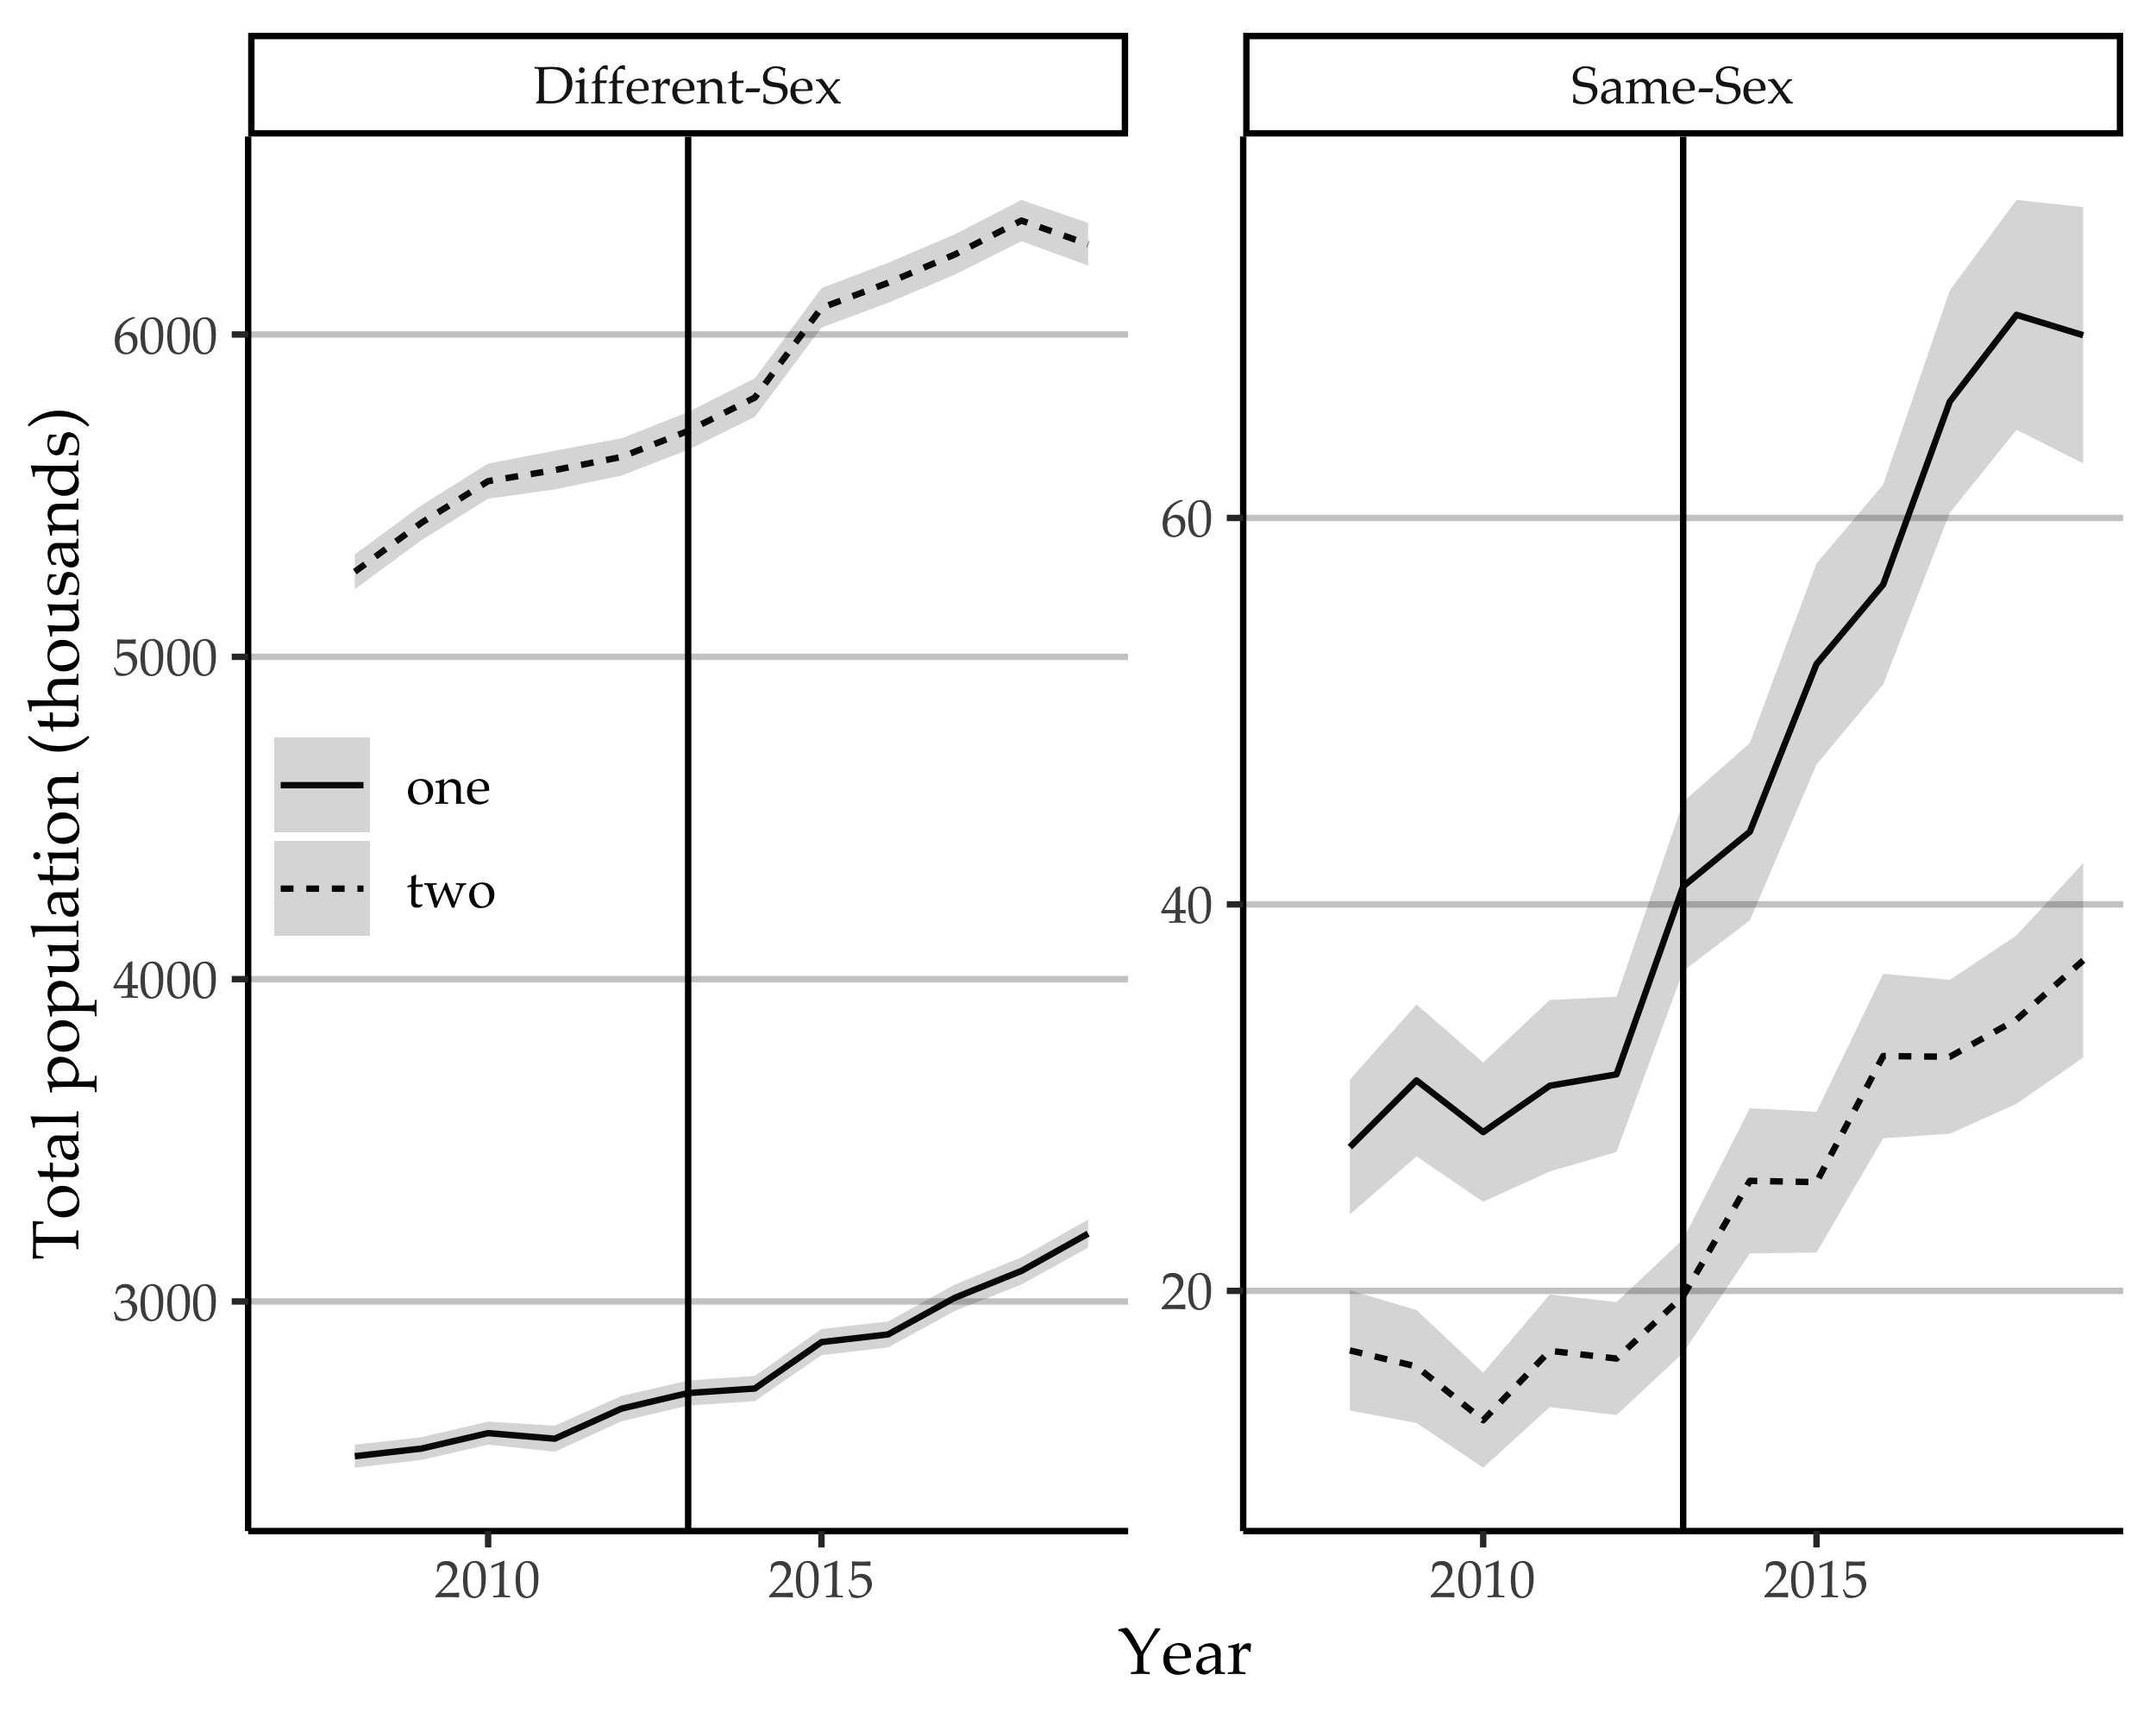
\includegraphics{ssimm_draft_files/figure-latex/total-pop-1.pdf}
\caption{\label{fig:total-pop}Estimated totals of different- and same-sex couples containing one or two immigrants, 2008-2019, with 95\% confidence intervals. Vertical line placed at the year 2013, when DOMA was overturned.}
\end{figure}

The federal environment governing immigration significantly changed after 2013. The U.S. Supreme Court opinion ruling the Defense of Marriage Act (DOMA) unconstitutional opened the door for more same-sex immigrant couples to enter the U.S. under the same process long-governing different-sex couples. Indeed, as Figure \ref{fig:total-pop} highlights, the number of same-sex immigrant couples in the U.S. grew significantly following this ruling -- especially when compared to different-sex couples. In 2013, there were 61 thousand. By 2019, this grew to 107 thousand. Aside from allowing gay and lesbian families to remain unified, this national opening created an important moment for the scholarly community as well. Now, more careful investigation into the factors both pushing and pulling same-sex immigrant couples into the U.S. can be conducted beyond idiosyncratic asylum claims. The present research fits squarely within this critical research gap.

\hypertarget{understanding-influences-on-migration-patterns}{%
\section{Understanding Influences on Migration Patterns}\label{understanding-influences-on-migration-patterns}}

\hypertarget{conventional-explanations}{%
\subsection{Conventional Explanations}\label{conventional-explanations}}

Our analysis compares conventional explanations for migration to political ones related to LGBT policy. These conventional explanations are frequently combined in a ``gravity model,'' which Anderson (\protect\hyperlink{ref-anderson_2011}{2011, p. 134}) describes in general terms: ``A mass of goods or labor or other factors of production supplied at origin \(i\), \(Y_i\), is attracted to a mass of demand for goods or labor at destination \(j\), \(E_j\), but the potential flow is reduced by the distance between them, \(d_{ij}\).'' This model continues to be widely applied to predict large-scale migration (\protect\hyperlink{ref-beine_2016}{Beine et al., 2016}; \protect\hyperlink{ref-karemera_2000}{Karemera et al., 2000}; \protect\hyperlink{ref-poot_2016}{Poot et al., 2016}).

Neoclassical economic theories motivate the traditional variables to include. Such theories posit that promise of material gain is a frequent motivation to migrate (\protect\hyperlink{ref-hatton_2005a}{Hatton \& Williamson, 2005}; \protect\hyperlink{ref-todaro_1980}{Todaro, 1980}); at the micro level, individuals who stand to gain greater returns to their education are more likely to migrate. At the macro level, these theories predict that migrants will follow wage and unemployment differentials across countries. Hence gravity models usually include difference in per capita GDP between sending and receiving countries. To account for migration costs, gravity models adjust for distance: immigrants are more likely to migrate between proximate countries, especially those that share a border.

Although the traditional gravity model focuses only on distance and economic ``mass,'' in recent years it has been refined with the incorporation of sociological theories of migration (\protect\hyperlink{ref-massey_1999}{Massey et al., 1999}), including political, cultural, and network variables (\protect\hyperlink{ref-fitzgerald_2014}{Fitzgerald et al., 2014}; \protect\hyperlink{ref-karemera_2000}{Karemera et al., 2000}; \protect\hyperlink{ref-mayda_2010}{Mayda, 2010}). Scholars have shown that shared language, colonial history, and democracy matter in the sending country, and immigrant rights matter in the receiving country. Recent models also highlight the importance of measures of immigrant networks, such as co-national immigrant stock (\protect\hyperlink{ref-beine_2016}{Beine et al., 2016}; \protect\hyperlink{ref-poot_2016}{Poot et al., 2016}). Though the incorporation of sociological theories into migration studies is a welcomed development, as mentioned, previous scholarship has not explicitly applied these analyses and insights into the migration of same-sex couples. Consequently, we do not know if these same patterns hold. But rather than offering a direct comparison into how these previous models apply to same-sex couples, we seek to intervene within migration scholarship by explicitly considering how sexuality, and the governence of it, additionally influence migration processes.

\hypertarget{our-intervention}{%
\subsection{Our Intervention}\label{our-intervention}}

Though migration scholarship typically emphasizes economic considerations as institutionalized in the gravity model, we argue that it is also imperative to take sexuality, and the state's role in governing sexuality, into account for understanding migratory patterns (\protect\hyperlink{ref-cantu_2009}{Cantú, 2009}; \protect\hyperlink{ref-carrillo_2018}{Carrillo, 2018}). One reason why this area of research has yet to be fully considered, in addition to previous restrictions outlined, is because the literature largely assumes immigrants are heterosexual or simply neglects to consider them as fully constitutive, diverse sexual beings (\protect\hyperlink{ref-canaday_2009}{Canaday, 2009}; \protect\hyperlink{ref-epstein_2014}{Epstein \& Carrillo, 2014}; \protect\hyperlink{ref-gonzalez-lopez_2005}{González-López, 2005}).

Consequently, analyses into how sexuality motivates migratory decisions or how migration reimagines sexual behaviors and understandings are limited (\protect\hyperlink{ref-carrillo_2018}{Carrillo, 2018}). Even more limited are explicit analyses into how policies such as same-sex marriage, hate crime protections, sodomy, and the like, further influence migration patterns. The nascent scholarship concerning queer migrants that does exist, though, suggests that policy environments are a central concern when making these decisions (\protect\hyperlink{ref-cantu_2009}{Cantú, 2009}; \protect\hyperlink{ref-luibheid_2005}{Luibhéid \& Cantú, 2005}). For example, (\protect\hyperlink{ref-nakamura_2017}{\textbf{nakamura\_2017?}}) interview same-sex couples who fled to Cananda due to the U.S.' lack of policies recognizing and affirming their relationships. Therefore, below, we theorize why LGBT policies at country-of-origin and residing U.S. state influence the push and pull of same-sex couples within the U.S.

Laws governing LGBT communities have significantly transformed. These changes are part of a broader global trend in which LGBT rights are increasingly incorporated within existing human rights frameworks -- pressuring countries to respond in turn (\protect\hyperlink{ref-velasco_2018}{Velasco, 2018}). These new dynamics have spurred research into understanding the causes of policy reforms and why countries have taken such varied approaches to enacting reform -- both in expanding rights but also further restricting them (\protect\hyperlink{ref-ayoub_2016}{Ayoub, 2016}). Only recently are scholars starting to understand the direct consequences of these changes on the lives of LGBT people (\protect\hyperlink{ref-boertien_2019}{Boertien \& Vignoli, 2019}; \protect\hyperlink{ref-carpenter_2020}{Carpenter, 2020}; \protect\hyperlink{ref-kail_2015}{Kail et al., 2015}). Though this emerging scholarship within the U.S. context focuses largely on health and well-being, particularly concerning marriage laws, there are several reasons why these new realities are likely to also influence migration outcomes.

Sexuality has long factored into migratory decisions. However, as the global awareness of LGBT rights expands, sexuality is increasingly a salient and important factor when deciding to leave one's home country (\protect\hyperlink{ref-mole_2018a}{Mole, 2018}; \protect\hyperlink{ref-murray_2016}{Murray, 2016}). Part of this is due to international organizations' construction of sexuality as a legitimate basis for leaving. For example, in 2008, the United Nations High Commissioner for Refugees issued a new guidance note for why and how countries should consider sexual orientation and gender identity when granting asylum claims. The note states:

\begin{quote}
``{[}I{]}ndividuals experience serious human rights abuses and other forms of persecution due to their actual or perceived sexual orientation and/or gender identity. While persecution of Lesbian, Gay, Bisexual, Transgender and Intersex (hereafter ``LGBTI'') individuals and those perceived to be LGBTI is not a new phenomenon, there is greater awareness in many countries of asylum that people fleeing persecution for reasons of their sexual orientation and/or gender identity can qualify as refugees {[}\ldots{]}.''
\end{quote}

The note continues to guide various authorities to consider discriminatory domestic policies when evaluating asylum claims as such policies ``can create or contribute to an oppressive atmosphere of intolerance and generate a threat of prosecution,'' (\protect\hyperlink{ref-unhcr_2008}{UNHCR, 2008, p. 8}). International organizations like the European Union and various countries have since followed (\protect\hyperlink{ref-giametta_2020}{Giametta, 2020}).

As globalization of LGBT rights increases, so too does the transnational flow of information, cultural content, and overall visibility (\protect\hyperlink{ref-ayoub_2016}{Ayoub, 2016}; \protect\hyperlink{ref-ayoub_2017}{Ayoub \& Garretson, 2017}). For example, access to gay characters in film and gay content on the Internet contributed toward Iranian refugees to seek sexual freedom and affirming political environments in the West (\protect\hyperlink{ref-karimi_2020}{Karimi, 2020}). Altogether, these developments in the global environment helped to shift sexuality, which has always been in the background of migratory decisions, to the foreground.

Despite this growing awareness of LGBT rights, countries vary greatly in their policy environments (\protect\hyperlink{ref-velasco_2020}{Velasco, 2020}). We theorize that country-of-origin policies shape migration into the U.S. by same-sex couples in two broad ways. First, as mentioned, migrants may seek to escape repressive contexts. As Adur (\protect\hyperlink{ref-adur_2018}{2018, p. 321}) states, ``sexuality also shapes migration as LGBTI immigrants relocate in pursuit of spaces that they \emph{imagine} will be safer and more liberal'' (emphasis theirs). Although the U.S. is certainly less progressive and inviting compared to many other Western states, high-profile developments such as marriage equality can contribute to an imagined openness. To date, queer migration research largely studies same-sex couples seeking to leave repressive conditions. Part of this is because of the U.S. policy environment which, for so long, did not define same-sex couples as ``family'' and left asylum as one of the few viable mechanisms for entry (\protect\hyperlink{ref-luibheid_2008}{Luibhéid, 2008}; \protect\hyperlink{ref-vogler_2016}{Vogler, 2016}). Similarly, another strand of research documents people in more oppressive contexts seeking out partners in more equitable locations who can then sponsor them through the immigration process (\protect\hyperlink{ref-carrillo_2018}{Carrillo, 2018}; \protect\hyperlink{ref-corey-boulet_2019}{Corey-Boulet, 2019}). These qualitative studies would suggest that immigrant same-sex couples are largely fleeing repressive contexts, but does this pattern hold more broadly?

Alternatively, same-sex couples from countries with greater recognition and access to sexuality-related rights and services may be in better positions to make such an important, and expensive, move. Long-standing research on immigrant selection demonstrates that migrants are typically from stronger social positions -- more formal education, higher incomes, and more prestigious occupations (\protect\hyperlink{ref-feliciano_2020}{Feliciano, 2020}). Given the high barriers to migrating, it is possible that same-sex couples are more likely to come from countries that have affirming and supportive policies in place, such as protections against employment discrimination or the legal and material benefits of marriage. Such policies enable and facilitate the employment security and the social and human capital necessary to navigate the immigration process. Additionally, being from a country where the state recognizes and validates one's sexuality and relationships may make such commitments more likely or may make survey respondents, once in the U.S., more comfortable disclosing such relationships.

While these country-of-origin policies may influence the ``push'' of same-sex couples out of their home country, the varied policy environments across U.S. states are likely to differentially ``pull'' these couples. Typically, a strong predictor of where migrants locate within the U.S. are network effects -- they locate where the people they know are located (\protect\hyperlink{ref-massey_1987}{Massey et al., 1987}; \protect\hyperlink{ref-palloni_2001}{Palloni et al., 2001}; \protect\hyperlink{ref-portes_1998}{Portes, 1998}). Existing research does highlight, though, that gay and lesbian couples within the U.S. were likely to leave states without marriage equality prior to national recognition (\protect\hyperlink{ref-beaudin_2017}{Beaudin, 2017}). If this results in a greater concentration of same-esx couples in states with marriage equality and other protective policies, it increases the chances that same-sex immigrant couples know someone in those states as well -- seeing as queer migrants often have strong cross-national networks that relay such information (\protect\hyperlink{ref-stella_2020}{Stella \& Gawlewicz, 2020}). Additionally, if migrants are coming from a country with greater legal protections, they are unlikely to want to relocate to a state where such rights are no longer recognized -- making the political environment acutely important. Of course, this is predicated on the assumption migrants take into account these sub-national variations -- which they very well may not do. Consequently, the ``pull'' to particular states may operate independently from specific state laws affirming LGB people and their relationships.

In sum, it is evident that sexuality, and the policies governing it, are extremely salient factors driving migratory decisions. Aside from qualitative examinations into queer migrants, especially asylum seekers, there is no large-\(N\) investigation into how the significant transformation of LGBT policies -- both globally and across U.S. states -- influence migration patterns in the U.S. Therefore, this research seeks to correct this gap within the literature by providing such an analysis and to further understand how the changing policy landscapes are differentially influencing the lives of queer people depending on their social positions.

\hypertarget{contrasting-the-demography-of-same-sex-and-different-sex-couples}{%
\subsection{Contrasting the Demography of Same-Sex and Different-Sex Couples}\label{contrasting-the-demography-of-same-sex-and-different-sex-couples}}

Prior to getting to the data and results of this analysis, it is first important to contextualize the present article within existing demographic scholarship. Previous demographic research suggests how characteristics salient to the migration process may differ between same- and different-sex couples. Cohabiting same-sex couples are more likely to reside in states in the Northeast and West, such as Vermont, Massachusetts, California, and Oregon (\protect\hyperlink{ref-gates_2013a}{Gates, 2013b}), that have often been at the forefront in safeguarding LGBT rights. The same-sex population is growing most rapidly, however, in the Midwest and South (\emph{ibid.}). Regardless of state, same-sex couples are more concentrated in urban areas, although this is more true for men than women (\protect\hyperlink{ref-baumle_2009}{Baumle et al., 2009}). This evidence suggests that immigrants in same-sex couples are also likely to choose progressive states and cities as their place of residence.

In the labor market, men in same-sex couples tend to earn less than their heterosexual counterparts, but women tend to earn more (\protect\hyperlink{ref-klawitter_2015}{Klawitter, 2015}). On average, married same-sex couples are older and have higher earnings than their different-sex counterparts (\protect\hyperlink{ref-fisher_2018}{Fisher et al., 2018}), while results for unmarried couples are mixed (\protect\hyperlink{ref-baumle_2009}{Baumle et al., 2009}). If immigrants in same-sex couples have higher earnings than heterosexual immigrants, then the typical push and pull factors of immigration may affect them differently. Same-sex couples also tend to be less homogamous in age, education, and race/ethnicity than their different-sex counterparts (\protect\hyperlink{ref-schwartz_2009}{Schwartz \& Graf, 2009}). Finally, although male same-sex romantic relationships generally have higher levels of instability than female or different-sex relationships (\protect\hyperlink{ref-joyner_2017}{Joyner et al., 2017}), the dissolution rates for cohabiting same- and different-sex couples are similar (\protect\hyperlink{ref-manning_2016}{Manning et al., 2016}). If LGB immigrants experience higher rates of union dissolution, then our estimates of the proportion of immigrants who are in same-sex couples represents a lower bound.

Note from Kris: I'm wondering if we should actually incorporate the ``labor market'' paragraph into the ``Conventional Explanations'' section? Put in there why we think conventional explanations apply/differ to same-sex couples? And then,the first paragraph could kinda go into theorizing why state policies may matter for same-sex couples but not different sex?

\hypertarget{data}{%
\section{Data}\label{data}}

\hypertarget{identifying-same-sex-couples-in-the-acs}{%
\subsection{Identifying Same-Sex Couples in the ACS}\label{identifying-same-sex-couples-in-the-acs}}

We merge individual-level data on immigrants in the U.S. with state- and country-level variables from a variety of datasets. The individual data come from the 2008 to 2019 ACS (\protect\hyperlink{ref-ruggles_2021}{Ruggles et al., 2021}). Each year, the ACS surveys a 1\% sample of the U.S. population about their education, occupation, income, family structure, immigration status, country of origin, location, and a variety of other individual and household attributes. We define a same-sex couple as two individuals of the same sex in the same household who report their relationship as ``spouse'' or ``unmarried partner.'' We limit the sample to individuals who immigrated at the age of 18 or older. The 11 years of survey data contain 9,119 same-sex couples that include at least one immigrant, for a total of 11,551 immigrants in same-sex couples with complete data. These immigrants are compared to 983,904 corresponding different-sex couples (containing 1,549,678 individual immigrants). Using these data, we construct different dependent variables, corresponding to the analysis of interest. Below, we outline how we utilize these data to construct dependent variables based on each analysis.

Measuring the prevalence of same-sex couples in the U.S. is difficult (\protect\hyperlink{ref-michaels_2013}{Michaels, 2013}). For one, identification of LGB individuals in data sources such as the ACS is only possible for those who self-identity as living with a same-sex spouse or unmarried partner (\protect\hyperlink{ref-baumle_2009}{Baumle et al., 2009, p. 6}). Since the surveys lack questions about sexual orientation, LGB individuals who do not live with a same-sex romantic partner or who do not feel comfortable with the partner labels of the ACS are not part of the analysis. In addition, some measurement error may result when different-sex couples accidentally misspecify the gender of one of the partners (\protect\hyperlink{ref-gates_2009a}{Gates, 2009}); beginning in 2008 the Census Bureau made changes to ACS gender and partnership questions in order to prevent such errors (\protect\hyperlink{ref-u.s.censusbureau_2013}{U.S. Census Bureau, 2013}), so we rely on data only from 2008 onward, but pitfalls remain.

In a Census Bureau working paper, \protect\hyperlink{ref-kreider_2015}{Kreider \& Lofquist} (\protect\hyperlink{ref-kreider_2015}{2015}) use personal information such as names and addresses match same-sex couples from the 2010 ACS to Social Security administrative data. They find that 58 percent of married couples coded as same-sex in the ACS are coded as different-sex in the administrative data. The corresponding sex mismatch rate for unmarried same-sex couples is 7 percent. (Our data include 4,633 married and 4,486 unmarried same-sex immigrant couples.) A follow-up study (\protect\hyperlink{ref-kreider_2017}{Kreider et al., 2017}) shows that these mismatch rates appear to have fallen: In a 2016 ACS test module that included explicit categories for different- and same-sex spouses and partners, 31 percent of married and 3 percent of unmarried same-sex couples had inconsistent sex responses. This decreasing mismatch rate may be due to the greater numbers of same-sex couples openly identifying themselves as well as the growing popularity of responding to the ACS via Internet (see Supplementary Material), a response mode introduced in 2013 which is now the default (\protect\hyperlink{ref-u.s.censusbureau_2017}{U.S. Census Bureau, 2017}). In the 2016 test of the ACS, the mismatch rate for mail-in responses was 47 and 6 percent for married and unmarried same-sex couples, respectively, whereas for Internet responses they were only 22 and 2.4 percent (\protect\hyperlink{ref-kreider_2017}{Kreider et al., 2017}).\footnote{An interview-based CATI/CAPI response mode is sometimes administered as well (to 15 percent of our sample of immigrants in same-sex couples), but the 2016 study did not assess its error rate. In the 2010 ACS, Kreider and Lofquist (2015) find CATI/CAPI sex reporting mismatch for 46 and 13 percent for married and unmarried same-sex couples, respectively.} In our sample of immigrants in same-sex couples, 4,630 responded by mail and 5,176 responded by Internet survey.

Despite these difficulties, many researchers have relied on ACS data to draw demographic conclusions about same-sex couples in the U.S., usually without making accommodations for measurement error (\protect\hyperlink{ref-boertien_2019}{Boertien \& Vignoli, 2019}; \protect\hyperlink{ref-gates_2013}{Gates, 2013a}; \protect\hyperlink{ref-giddings_2014}{Giddings et al., 2014}; \protect\hyperlink{ref-goldberg_2021}{Goldberg \& Conron, 2021}; e.g. \protect\hyperlink{ref-poston_2017}{Poston et al., 2017}). In several ways, we test the sensitivity of our results, especially to the possibility that a large proportion of apparently same-sex couples misreported a partner's sex. However, such adjustments assume that sex response error occurs randomly throughout the immigrant population. Beginning in 2019, the ACS added explicit ``opposite-sex'' and ``same-sex'' categories to the relationship questions, so future work on same-sex couples in the ACS will be more reliable (\protect\hyperlink{ref-goodnature_2021}{Goodnature \& Neto, 2021}).

\hypertarget{explanatory-variables}{%
\subsection{Explanatory Variables}\label{explanatory-variables}}

Our explanatory variables of interest are the LGBT policy contexts in country-of-origin and U.S. state of residence. To create the U.S. state policy index, we compile data from the Movement Advancement Project, a leading LGBT organization in the U.S. that collects data on a number of relevant policies. Our state index encompasses both progressive policies (full marriage equality, state recognition of civil unions and domestic partnerships, ban on all employment and housing discrimination based on sexual orientation, hate crime protections based on sexual orientation, legal joint adoption by same-sex couples, and a ban on conversation therapy for minors) and regressive policies (criminalization of sodomy, state constitutional bans of marriage equality, religious freedom exemptions to discriminate against same-sex couples in adoption, and state-level bans on local non-discrimination ordinances encompassing sexual orientation). The state index ranges from -1 to 7, and the mean score of country of origin for immigrants in our sample is 3.2.

We measure the origin country policy environment using the LGBT Policy Index (\protect\hyperlink{ref-velasco_2018}{Velasco, 2018}). This index comprises 14 policies, many similar to those above, but including additional policies like the death penalty for homosexual acts, propaganda laws limiting free speech for LGBT communities, and equal age of consent between same-sex and opposite-sex couples. Both indices are created by summing the net total of progressive policies (scored \(+1\)) over regressive policies (scored \(-1\)). The state index ranges from -3.2 to 11, and the mean score of country of origin for immigrants in our sample is 1.7.

Immigrants are assigned U.S. state index scores based on their state of residence as reported in the ACS. They are assigned country-of-origin index scores based on their year of immigration. Since the country policy index begins at 1991, we anyone who immigrated before 1991 gets assigned the 1991 value.\footnote{In additional models, not shown, we limit the sample only to those who immigrated in 1991 or after tather than assigning those who immigrated prior to 1991 their country value at 1991. Results are substantively similar and available upon request}

Aside from the country and state indices, we also include a binary variable to indicate the change in national policy environment within the U.S. following the overturning of DOMA. This represents an important shift opening up traditional pathways of immigration to same-sex couples. We also include an interaction term between this post-DOMA indicator and country-of-origin index because we theorize that the effects will be more pronounced following this period.

\hypertarget{control-variables}{%
\subsection{Control Variables}\label{control-variables}}

Our country- and state-level controls come from a variety of sources. Country-of-origin controls for bilateral distance, contiguous border, common official language, common ethnic language, and whether the country was a former colony of the U.S. come from CEPII's GeoDist dataset (\protect\hyperlink{ref-mayer_2011}{Mayer \& Zignago, 2011}). Difference in wages, calculated as difference in per capita GDP at purchasing power parity, come from the Penn World Table (\protect\hyperlink{ref-feenstra_2015}{Feenstra et al., 2015}), and we rely on World Bank data for differences in unemployment rates (\protect\hyperlink{ref-worldbank_2020}{World Bank, 2020}). We use Polity5 measures of democratization of the country of origin (\protect\hyperlink{ref-marshall_2018}{Marshall, 2018}), with linear interpolation for missing years. We proxy network effects by dividing each country's immigrant stock by the total number of immigrants in the U.S. in a given year, using the World Bank's Global Bilateral Migration Database (\protect\hyperlink{ref-ozden_2011}{Özden et al., 2011}) for 1960, 1970, and 1980 and the UN's Trends in International Migrant Stock report for (\protect\hyperlink{ref-unitednations_2017}{United Nations, 2017}) for 1990, 1995, 2000, 2005, 2010, 2015, and 2017, linearly interpolating to yield an annual time series from 1960 to 2020. For state controls, we use per capita income by year from the Bureau of Economic Analysis (\protect\hyperlink{ref-bea_2020}{BEA, 2020}) and state-level annual unemployment rates from the Bureau of Labor Statistics (\protect\hyperlink{ref-bls_2020}{BLS, 2020}). All monetary variables are adjusted to 1999 U.S. dollars.

For our individual-level analysis we include individual controls from the ACS for reported sex, age, education (with categories for less than high school, high school, some college, and college), year of immigration, log positive income, and a binary indicator for income reported to be 0 or less.

\hypertarget{analytic-strategy}{%
\section{Analytic Strategy}\label{analytic-strategy}}

Our first goal is to isolate the effects of country-of-origin LGBT policy on the immigration of immigrants in same-sex couples. The ideal survey would follow potential immigrants over time and have information about sexual orientation, allowing us to estimate how the probability of migrating and choice of U.S. state of residence vary by sexual orientation. This ideal dataset does not exist, but we approximate it at the macro level. We take the number of immigrants in same-sex couples from a given country and a given year of immigration and divide by the total number of immigrants from that country-year. We then multiply by 100 to yield a percentage. In effect this controls for aspects of the migration process common to all immigrants from a given country; if sending-country LGBT policy has no effect on migration rates of LGB immigrants, then we would expect these proportions to be similar across countries. However, even if proportions of immigrants in same-sex couples vary between countries, LGBT policy may not be the cause; perhaps LGB immigrants respond idiosyncratically to gravity-model variables that may covary with LGBT policy, such as country income, unemployment, democratization, relationship to the U.S., and immigrant networks, so we control for these variables in our preferred model and estimate using ordinary least squares (OLS) regression. Our preferred model also includes country fixed effects to account for unobserved heterogeneity within countries. All of these models use country-clustered standard errors. To assess the influence of the 2013 Supreme Court decision on DOMA, we also add a dichotomous variable for whether the year of immigration was later than 2013.

Our next set of models focus on U.S. state LGBT policy. We reshape the data so that each observation is the proportion of immigrants in same-sex couples from country \(x\) in state \(y\) in year \(z\), then multiply by 100. As in the previous set of models, this reshaping acts to control for aspects of migrant settlement common to immigrants from the same country. We regress this proportion on state and sending-country policy scores, controlling for the same country-level attributes as in the previous set of models and adding state-level controls for per capita income and unemployment rate. We include state and country-of-origin fixed effects, and we cluster errors at the state level.

Our final set of models turns toward the individual: conditional on immigrating to the U.S., do immigrant in same-sex couples choose more LGBT-friendly states to reside in? And how does sending-country LGBT context moderate this relationship? This part of the analysis uses ordered logistic regression to predict the policy index of state of residence. Whereas the full U.S. state policy index ranges from -1 to 7, we break up the index into three ``bins'': repressive (0 and less), neutral (1 or 2), and progressive (3 and greater). We regress this ordered categorical outcome on a same-sex indicator and country-of-origin policy score, interacting these variables in our preferred model. The interaction term estimates the possibly moderating effect of origin-country policy context. We also control for individual attributes that could possibly confound our results, interacting these with the same-sex indicator, and we include survey-year fixed effects and country-clustered standard errors.

\hypertarget{results}{%
\section{Results}\label{results}}

\hypertarget{descriptive-statistics}{%
\subsection{Descriptive statistics}\label{descriptive-statistics}}

We first estimate total numbers of immigrants in same- and different-sex couples, applying survey weights to obtain population-level estimates from the ACS. Figure \ref{fig:total-pop} shows that whereas numbers of different-sex immigrant couples have steadily increased over the period of study, numbers of same-sex immigrant couples have increased much more rapidly, especially since the the 2013 Supreme Court decision overturning DOMA.

\begin{figure}
\centering
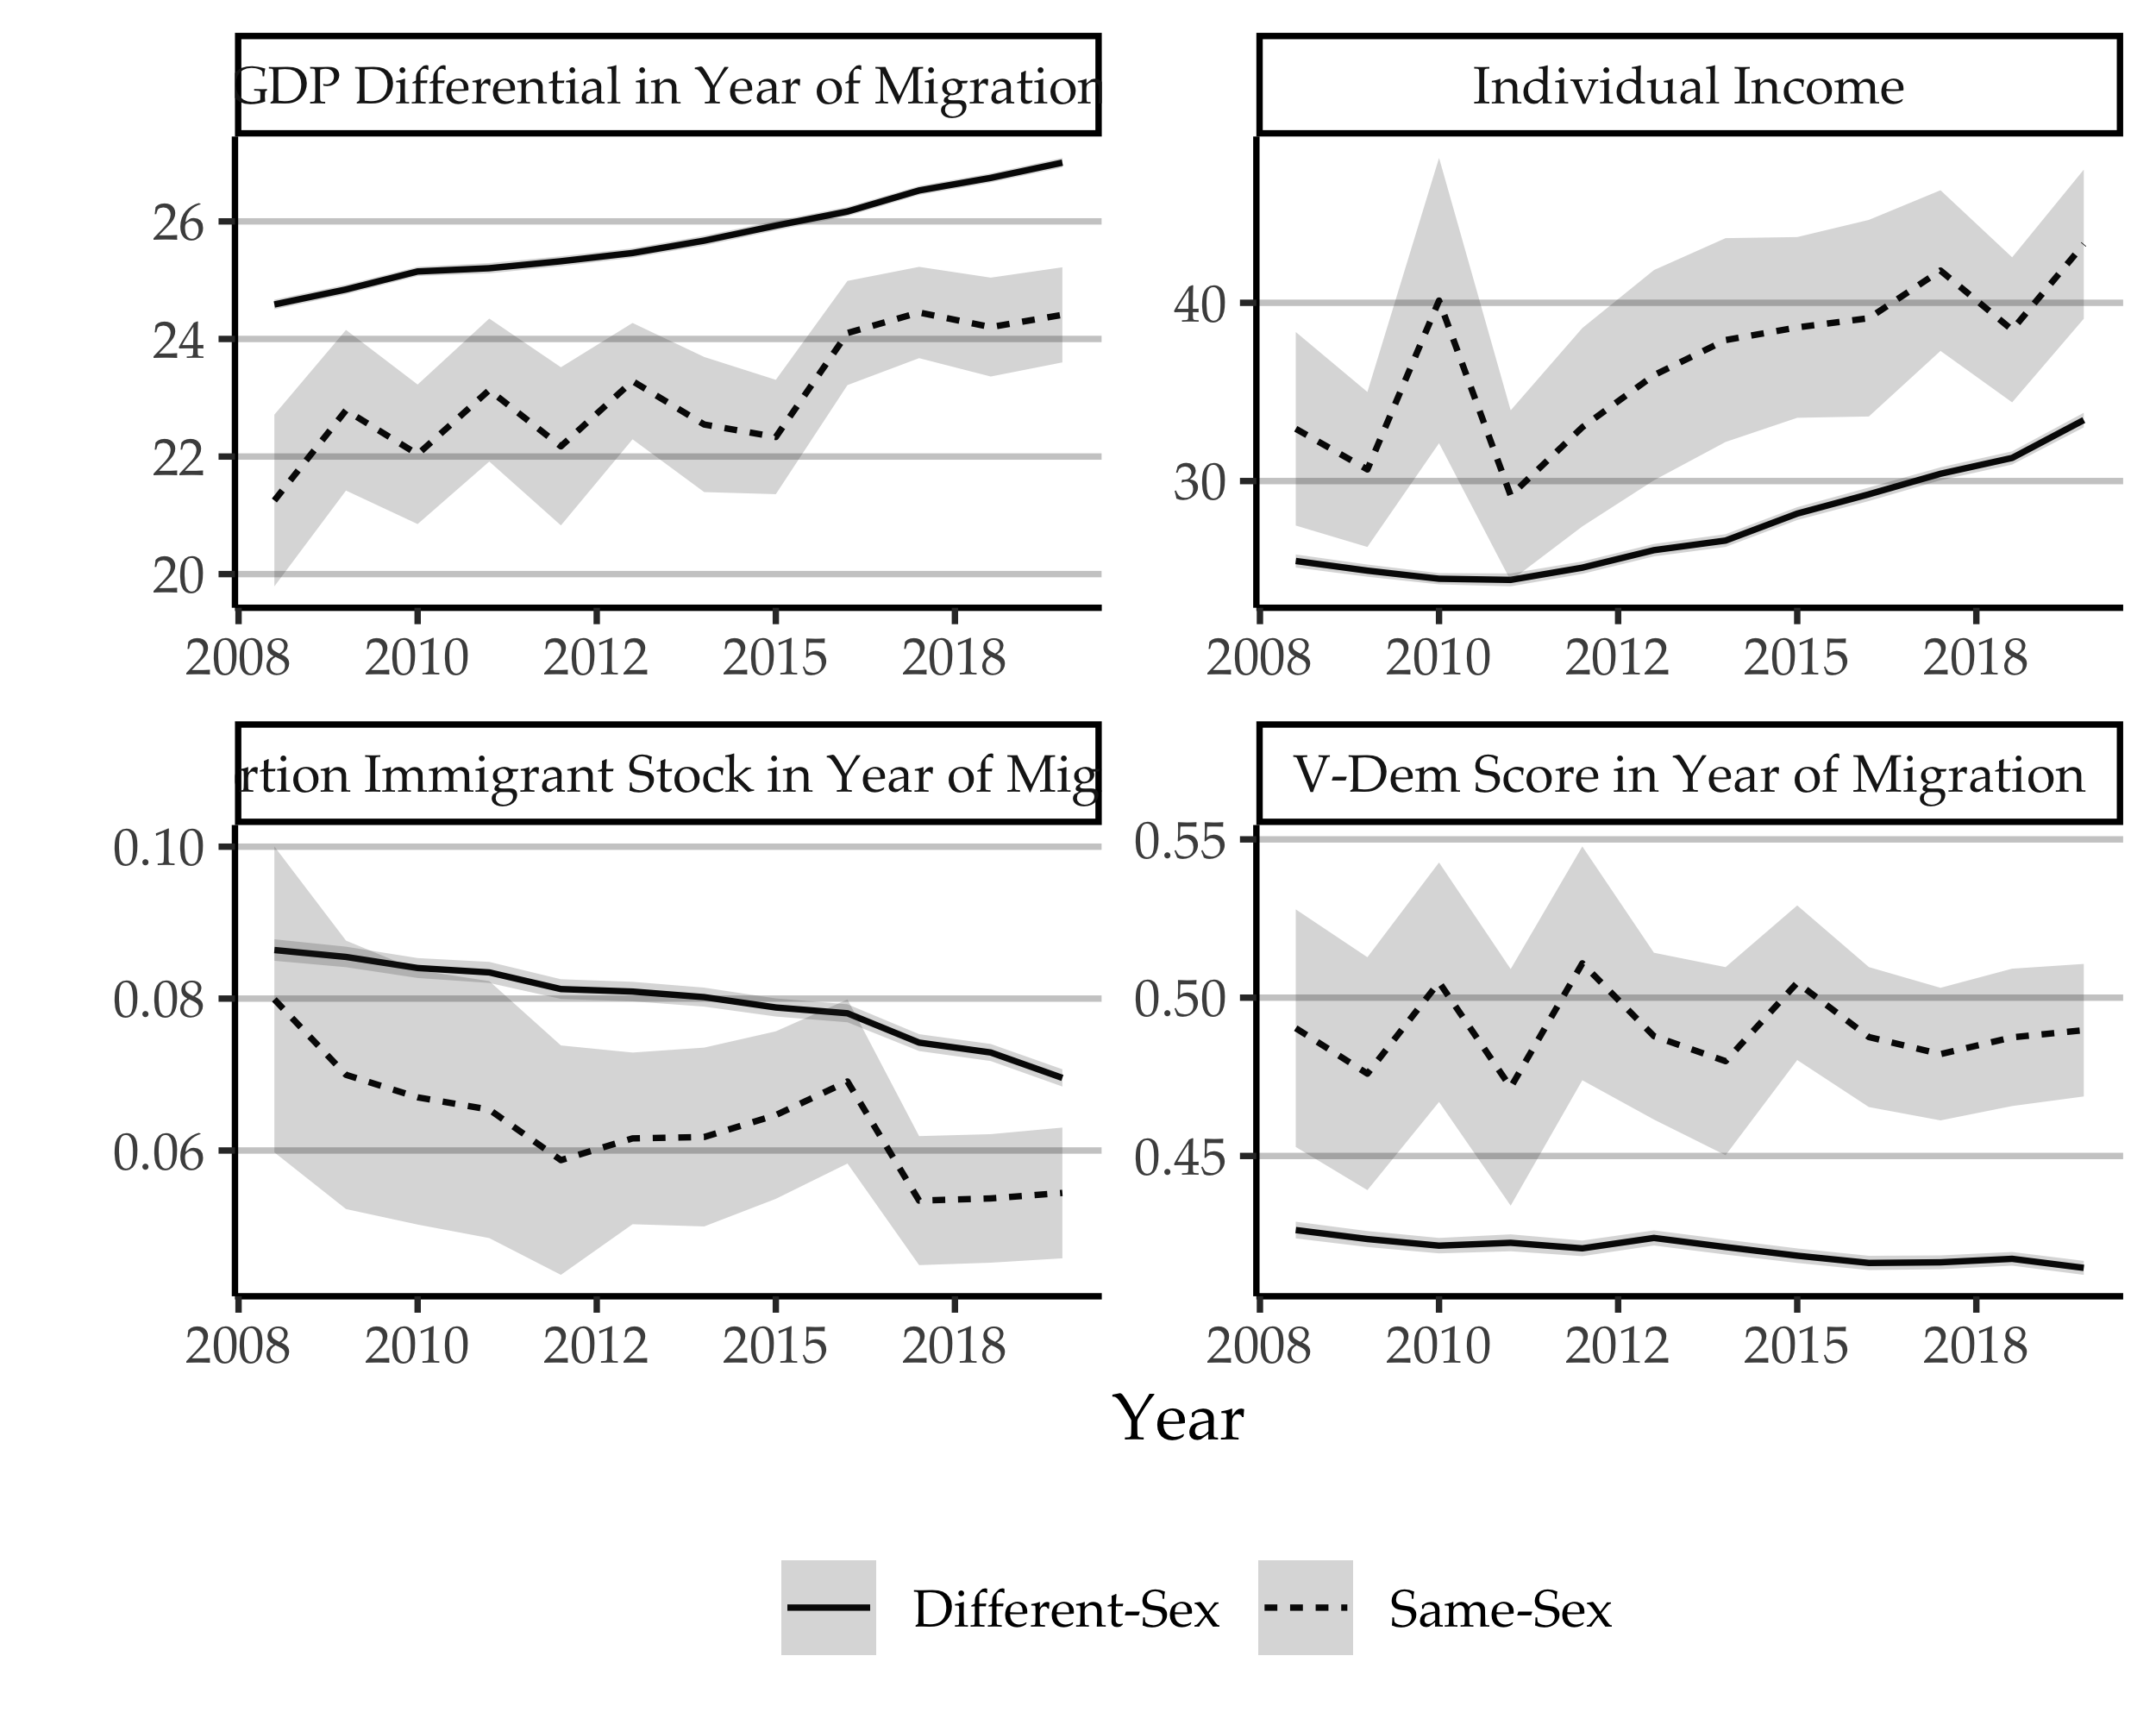
\includegraphics{ssimm_draft_files/figure-latex/desc-1.pdf}
\caption{\label{fig:desc}Descriptive statistics for immigrants in couples 2008-2019, with survey weights and 95\% confidence intervals. All currency in 1000s of 1999 dollars.}
\end{figure}

How do same- and different-sex immigrant couples differ in their individual attributes? Do variables typically used in ``gravity models'' for migration differ between the groups? Figure \ref{fig:desc} compares immigrants in same- and different-sex couples on four variables. First, macroeconomic theory predicts that difference in wages across countries is one of the most important motivations for migration. The first panel in Figure \ref{fig:desc} shows that the wage differential is indeed positive for both groups of immigrants, but it is significantly more positive for immigrants in different-sex couples. Statistics for the unemployment rate differential (not shown) indicate similar trends: LGB immigrants come from countries with lower unemployment rates. These findings indicate that macroeconomic considerations may be less important to the migration of LGB immigrants. The second panel corroborates this finding on the individual level: not only do immigrants in same-sex couples come from countries with higher per capita GDP, but they individually tend to earn more than immigrants in different-sex couples. Additional analyses (not shown) demonstrate that immigrants in same-sex couples also tend to work in professions with higher occupational prestige scores and have somewhat higher education qualifications, indicating that they may come from more privileged social origins than their heterosexual counterparts.

Panel three of Figure \ref{fig:desc} compares democracy level of country of origin at time of migration for immigrants in our study. We see that levels of democracy tend to be higher for immigrants in same-sex couples, indicating that political context may play a more important or different role in their migration. Finally, the fourth panel of Figure \ref{fig:desc} looks at a measure of network effects: at the time of immigration, what is the proportion of total immigrants in the U.S. from the country of origin of members of our sample? Compared to different-sex couples, immigrants in same-sex couples immigrated from countries that were less represented in the U.S. population at the time of migration. This indicates that the network effects that attract migrants from the same country of origin may be less relevant to LGB immigrants.

Although we see significant differences between same- and different-sex couples on a number of important migration variables, none shows the sudden jump in recent years reflected in Figure \ref{fig:total-pop}. Turning to LGBT policy may better explain this surge. Figure \ref{fig:policy-desc} charts the average country-of-origin and U.S.-state LGBT policy score for the immigrants in our sample over time, comparing means for immigrants in same- and different-sex couples. The left panel shows that country-of-origin index at time of migration is generally higher for immigrants in same-sex couples, and since 2013 it has rapidly increased. Immigrants in same-sex couples tend to come from more progressive countries, and this trend tracks closely with the overall population of this group. The right panel indicates less of a difference in U.S. state policies, although states where immigrants in same-sex couples live tend to score somewhat higher.

\begin{figure}
\centering
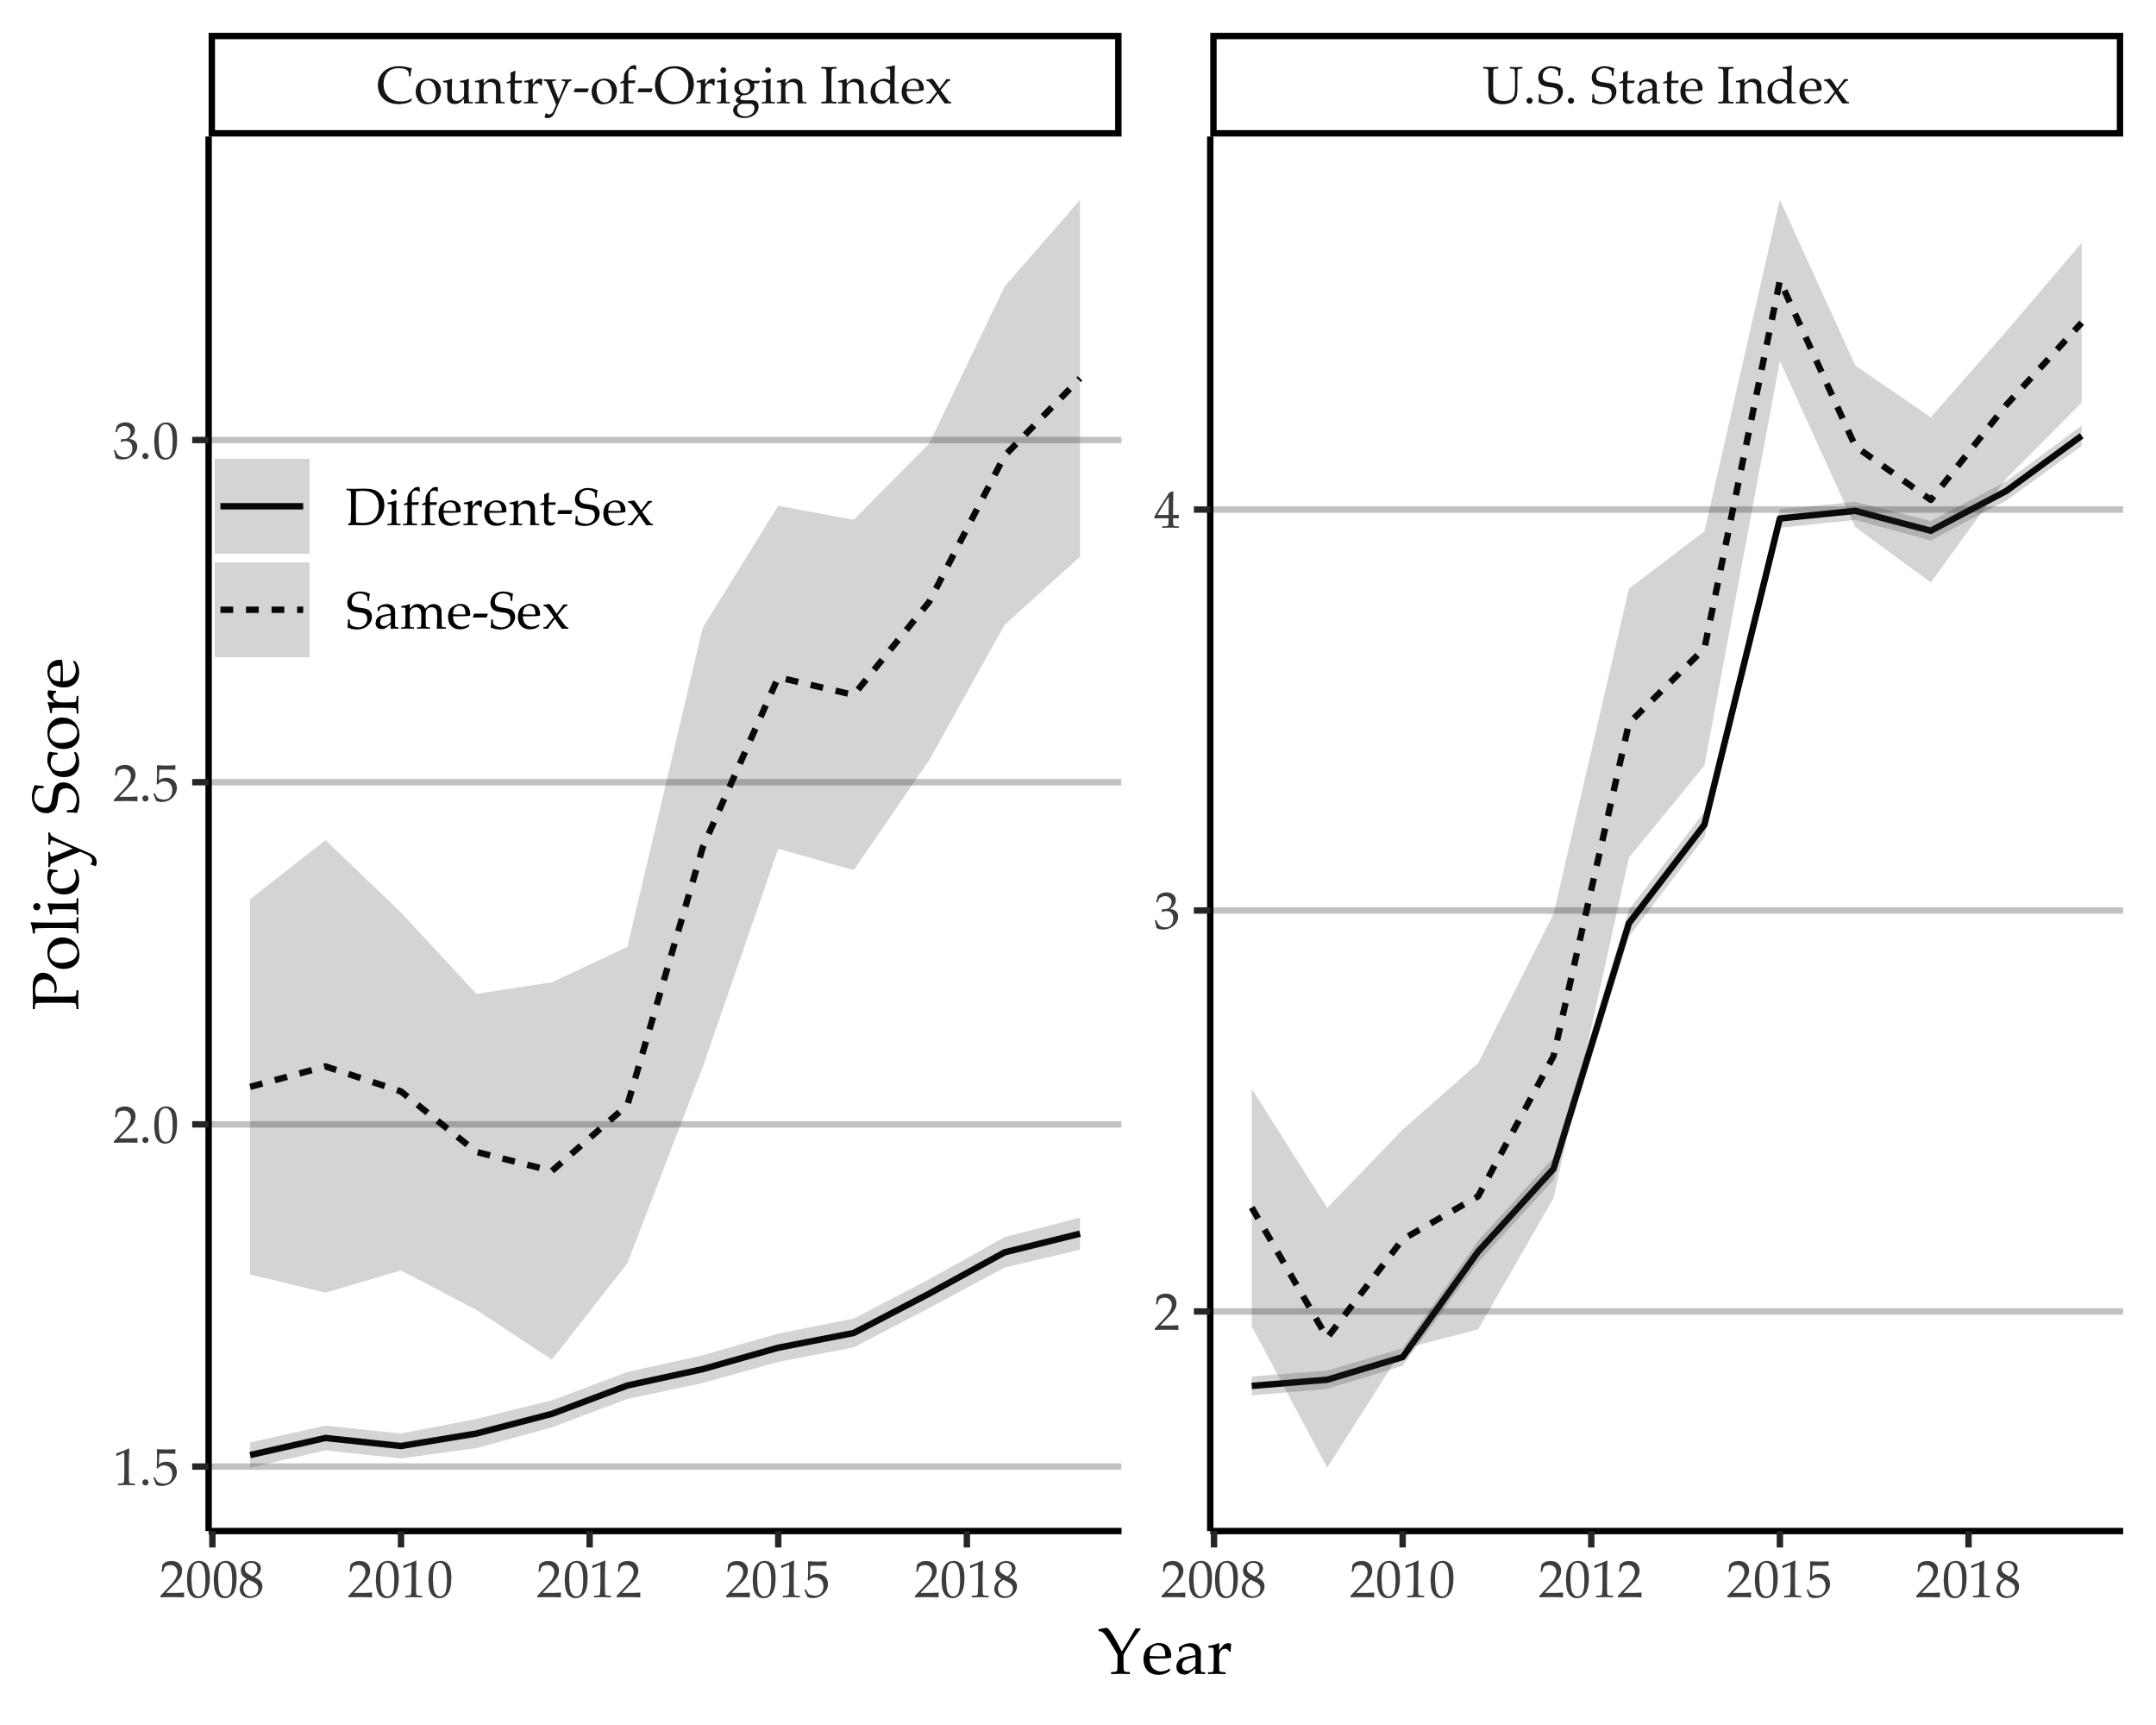
\includegraphics{ssimm_draft_files/figure-latex/policy-desc-1.pdf}
\caption{\label{fig:policy-desc}Mean country-of-origin and U.S. state policy index score for immigrants in same- and different-sex couples, 2008-2019, with 95\% confidence intervals.}
\end{figure}

\begin{table}

\caption{\label{tab:country-tab}Sending countries ranked by proportion immigrant couples with same-sex partners}
\centering
\begin{tabular}[t]{lllr}
\toprule
Rank & Country of origin & Proportion same-sex & Mean policy score\\
\midrule
1 & Australia & 2.51 \% & 4.07\\
2 & Mongolia & 2.37 \% & 2.25\\
3 & Belgium & 2.2 \% & 4.97\\
4 & Singapore & 2.12 \% & -0.20\\
5 & Netherlands & 2.06 \% & 7.15\\
6 & Malaysia & 2.05 \% & -0.89\\
7 & New Zealand & 2.04 \% & 5.43\\
8 & France & 2.02 \% & 6.06\\
9 & Zimbabwe & 2.01 \% & -0.95\\
10 & Spain & 1.95 \% & 5.57\\
\bottomrule
\multicolumn{4}{l}{\rule{0pt}{1em}\textit{Source:} American Community Survey 2008-2019. Authors' calculations.}\\
\end{tabular}
\end{table}

\begin{table}

\caption{\label{tab:state-tab}States ranked by proportion immigrant couples with same-sex partners}
\centering
\begin{tabular}[t]{lllr}
\toprule
Rank & State & Proportion same-sex & Mean policy score\\
\midrule
1 & Vermont & 2.10 \% & 5.17\\
2 & Maine & 1.56 \% & 4.79\\
3 & Montana & 1.47 \% & 0.80\\
4 & Missouri & 1.11 \% & 1.91\\
5 & Massachusetts & 1.10 \% & 4.77\\
6 & New York & 1.08 \% & 4.85\\
7 & Florida & 0.99 \% & 0.91\\
8 & New Hampshire & 0.95 \% & 4.33\\
9 & Mississippi & 0.94 \% & -0.49\\
10 & Minnesota & 0.92 \% & 4.63\\
\bottomrule
\multicolumn{4}{l}{\rule{0pt}{1em}\textit{Source:} American Community Survey 2008-2019. Authors' calculations.}\\
\end{tabular}
\end{table}

Table \ref{tab:country-tab} ranks the proportion of U.S. immigrants in same-sex couples based on country of origin, averaging over the 11 years of survey data. The top sending countries mostly held more progressive policies in year of departure for immigrants in our sample, but Singapore, Malaysia, and Zimbabwe maintained generally repressive policies. Table \ref{tab:state-tab} similarly ranks U.S. state by the proportion of immigrants in same-sex couples, averaging over the period of interest. Although states with progressive policies make the top of the list, somewhat repressive Mississippi lands at rank 8, and Montana, Missouri, and Florida still make the list with more neutral policies.

\hypertarget{model-results}{%
\subsection{Model Results}\label{model-results}}

Our first set of models predicts the percent of immigrants in same-sex couples by country of origin and year of immigration (Table \ref{tab:country-props}). Model 1 regresses this proportion on only our variable of interest: LGBT policy score in country of origin. We see that countries with more progressive LGBT policy tend to send more immigrants to the U.S. who end up in same-sex couples. The average country-level proportion of immigrants in same-sex couples is only 0.51 percent, so an increase of 0.079 per point increase in LGBT policy score represents a substantive effect.

Models 2 and 3 in Table \ref{tab:country-props} assess the robustness of this finding. Model 2 includes traditional controls from gravity models of immigration along with a measure of democratization and one of immigrant networks. The coefficient for country-of-origin score reduces slightly but remains highly significant. Notably, it is estimated to be more than twice the effect size of democratization score; the LGBT policy environment matters much more than the overall progressiveness of government policy. Model 3 includes country-of-origin fixed effects. Although in the fixed effects model coefficient for origin score is reduced by half compared to Model 1, it remains statistically significant.

\begin{table}[!htbp] \centering 
  \caption{OLS regressions of percent of immigrants in same-sex couples by year of immigration and country of origin. Country-clustered standard errors shown in parentheses. Country controls include population-weighted distance, contiguous border, common official language, common ethnic language, colonial relationship, wage differential, unemployment differential, proportion same-country stock, and Polity 5 measure of democratization.} 
  \label{tab:country-props} 
\begin{tabular}{@{\extracolsep{5pt}}lcccccc} 
\\[-1.8ex]\hline 
\hline \\[-1.8ex] 
 & \multicolumn{6}{c}{\textit{Dependent variable:}} \\ 
\cline{2-7} 
\\[-1.8ex] & \multicolumn{5}{c}{Percent in same-sex couples} & Married \\ 
\\[-1.8ex] & (1) & (2) & (3) & (4) & (5) & (6)\\ 
\hline \\[-1.8ex] 
 Country LGBT policy score & 0.079$^{***}$ & 0.046$^{***}$ & 0.042$^{**}$ & 0.019 & $-$0.017 & 0.010 \\ 
  & (0.008) & (0.010) & (0.015) & (0.016) & (0.019) & (0.017) \\ 
  & & & & & & \\ 
 Polity5 democratization &  & 0.023$^{***}$ & 0.004 & 0.0005 & 0.004 & 0.008 \\ 
  &  & (0.005) & (0.010) & (0.010) & (0.010) & (0.009) \\ 
  & & & & & & \\ 
 Post-2013 &  &  &  & 0.250$^{***}$ & 0.083 & 0.140$^{†}$ \\ 
  &  &  &  & (0.067) & (0.081) & (0.072) \\ 
  & & & & & & \\ 
 Country score × Post-2013 &  &  &  &  & 0.064$^{***}$ & 0.060$^{***}$ \\ 
  &  &  &  &  & (0.017) & (0.015) \\ 
  & & & & & & \\ 
\hline \\[-1.8ex] 
Country controls? & no & yes & yes & yes & yes & yes \\ 
Country FEs? & no & no & yes & yes & yes & yes \\ 
Observations & 3,222 & 3,222 & 3,222 & 3,222 & 3,222 & 3,222 \\ 
\hline 
\hline \\[-1.8ex] 
\multicolumn{7}{l}{Note: †p<0.1; *p<0.05; **p<0.01; ***p<0.001} \\ 
\multicolumn{7}{l}{Source: American Community Survey 2008-2019} \\ 
\end{tabular} 
\end{table}

Models 4, 5, and 6 in Table \ref{tab:country-props} assess how the 2013 Supreme Court decision striking down DOMA figures into these processes. Model 4 is the same as Model 3, but with a dichotomous ``Post-2013'' variable added. The influence of sending-country policy loses its significance in this model: 2013 was a significant turning point for LGB immigrants to the U.S., with the average representation from a given country growing by a quarter of a percent. Model 5 adds an interaction between sending-country LGBT policy score and the post-2013 dichotomous variable. This variable is significant and positive, while the other variables of interest lose significance. Sending-country policy and the post-2013 era both matter, but only in tandem: Only LGB immigrants from progressive countries see a boost in representation after the DOMA decision.

Finally, Model 6 restricts the sample to only married same-sex couples. Since the DOMA decision permitted visa sponsorship for same-sex spouses, this is subpopulation in which we would expect to see the greatest discontinuity pre- and post-2013. Indeed, for immigrants married to same-sex spouses the post-2013 variable and its interaction with sending-country policy score are both significant and positive. Although before 2013 progressive countries did not send more same-sex married couples, after 2013 these numbers grew sharply, and more progressive countries received an extra boost.

\begin{table}[!htbp] \centering 
  \caption{Percent same-sex in by country of origin, U.S. state, and survey year. Country-clustered standard errors are shown in parentheses. State controls include unemployment rate and per-capita income. Country controls include population-weighted distance, contiguous border, common official language, common ethnic language, colonial relationship, wage differential, unemployment differential, proportion same-country stock, and Polity 5 measure of democratization.} 
  \label{tab:state-props} 
\begin{tabular}{@{\extracolsep{5pt}}lcccc} 
\\[-1.8ex]\hline 
\hline \\[-1.8ex] 
 & \multicolumn{4}{c}{\textit{Dependent variable:}} \\ 
\cline{2-5} 
\\[-1.8ex] & \multicolumn{4}{c}{Percent in same-sex couples} \\ 
\\[-1.8ex] & (1) & (2) & (3) & (4)\\ 
\hline \\[-1.8ex] 
 State LGBT policy score & 0.035$^{*}$ & 0.041$^{*}$ & 0.019 & 0.034 \\ 
  & (0.018) & (0.018) & (0.034) & (0.034) \\ 
  & & & & \\ 
 Country LGBT policy score &  & 0.050$^{***}$ & 0.048$^{***}$ & 0.130$^{***}$ \\ 
  &  & (0.011) & (0.011) & (0.040) \\ 
  & & & & \\ 
\hline \\[-1.8ex] 
State controls and FEs? & no & no & yes & yes \\ 
Country controls and FEs? & no & no & no & yes \\ 
Observations & 39,458 & 39,458 & 39,458 & 39,458 \\ 
\hline 
\hline \\[-1.8ex] 
\multicolumn{5}{l}{Note: †p<0.1; *p<0.05; **p<0.01; ***p<0.001} \\ 
\multicolumn{5}{l}{Source: American Community Survey 2008-2019} \\ 
\end{tabular} 
\end{table}

We next turn to the effects of U.S. state LGBT policy. Table \ref{tab:state-props} presents models of U.S. state-level proportion of immigrants in same-sex couples, from a given country of origin in a given survey year. Model 1 contains only one predictor: U.S. state policy score in the survey year. We see that, on average, states with more friendly LGBT policies have somewhat higher proportions of immigrants in same-sex couples. Model 2 adds a predictor for country-of-origin policy score at the mean year of immigration. Although the coefficient for country of origin score is more precisely estimated, the two variables have effects of roughly equal size. A 2-point (one-standard deviation) increase origin score is associated with a 0.098 percentage-point increase of immigrants in same-sex couples, whereas the corresponding state policy standard deviation increase of 2.4 points is 0.1 percentage points.

According to the descriptive analysis above, immigrants in same-sex couples tend to have higher incomes and hold more prestigious occupations than immigrants in different-sex couples. This implies that immigrants in same-sex couples may be attracted to progressive states for their economic rather than political benefits, so Model 3 adds state-level controls and fixed effects. Indeed, in this model, the coefficient for state policy is reduced and rendered insignificant. Model 4 adds country-of-origin controls and fixed effects. The state policy effect remains imprecisely estimated, but country-of-origin policy has increased in strength. More progressive sending countries are represented by greater proportions of same-sex couples, while U.S. state policy appears to have little influence on their settlement patterns, at least in aggregate proportions.

\begin{table}[!htbp] \centering 
  \caption{Individual ordered logit analysis of three-category state policy score. Country-clustered standard errors are shown in parentheses. Individual controls include sex, age, education, number of children, log(income), indicator for no income, and year of immigration, which are all interacted with the indicator for same-sex couple.} 
  \label{tab:ord} 
\begin{tabular}{@{\extracolsep{5pt}}lccc} 
\\[-1.8ex]\hline 
\hline \\[-1.8ex] 
 & \multicolumn{3}{c}{\textit{Dependent variable:}} \\ 
\cline{2-4} 
\\[-1.8ex] & \multicolumn{3}{c}{Binned state LGBT policy score} \\ 
\\[-1.8ex] & (1) & (2) & (3)\\ 
\hline \\[-1.8ex] 
 Same-sex & 0.160$^{***}$ & 0.100$^{***}$ & 19.000$^{***}$ \\ 
  & (0.020) & (0.027) & (0.0004) \\ 
  & & & \\ 
 Country LGBT policy score &  & $-$0.051$^{***}$ & $-$0.022$^{***}$ \\ 
  &  & (0.003) & (0.003) \\ 
  & & & \\ 
 Same-sex × country score &  & 0.039$^{***}$ & 0.051$^{***}$ \\ 
  &  & (0.008) & (0.009) \\ 
  & & & \\ 
\hline \\[-1.8ex] 
Survey year FEs? & yes & yes & yes \\ 
Individual controls? & no & no & yes \\ 
Observations & 111,551 & 111,551 & 111,551 \\ 
\hline 
\hline \\[-1.8ex] 
\multicolumn{4}{l}{Note: †p<0.1; *p<0.05; **p<0.01; ***p<0.001} \\ 
\multicolumn{4}{l}{Source: American Community Survey 2008-2019} \\ 
\end{tabular} 
\end{table}

Our final set of models focuses on the individual. Conditional on migrating to the U.S., do immigrants in same-sex couples choose to live in more progressive states than their heterosexual counterparts? Table \ref{tab:ord} presents ordered logit models predicting whether an individual partnered immigrant lives in a U.S. state with repressive, neutral, or progressive LGBT policies, pooling data across survey years. Model 1 includes only one regressor: an indicator for whether the immigrant is in a same-sex couple. The positive coefficient indicates that immigrants in same-sex couples indeed tend to live in states with more LGBT-friendly policies. The predicted probability for an immigrant in a different-sex couple to live in a state with progressive LGBT policies is 0.6, whereas the corresponding probability for those in same-sex couples is 0.63. At the repressive end of the policy spectrum, the predicted probabilities are 0.22 and 0.2 for different- and same-sex couples, respectively.

How does country-of-origin context mediate this results? Model 2 adds sending-country LGBT policy score at the time of immigration to the regression, interacting it with the same-sex indicator. The coefficient for the same-sex indicator remains positive and significant, but we see opposite effects of the origin-score coefficient for immigrants in different- and same-sex couples. For different-sex couples, hailing from a more progressive country is associated with living in a more repressive U.S. state. For same-sex couples, the result is in the opposite direction: those from progressive countries tend to live in more progressive U.S. states.

Model 3 controls for possible individual confounders, interacting them with the same-sex indicator. If immigrants in same-sex couples also tend to have more education, higher income, different family structures, or less years of age, they may be choosing more progressive states due to other policies or economic conditions. As shown in Table \ref{tab:ord}, our variables of interest remain strong and in the same directions in this final model.

\begin{figure}
\centering
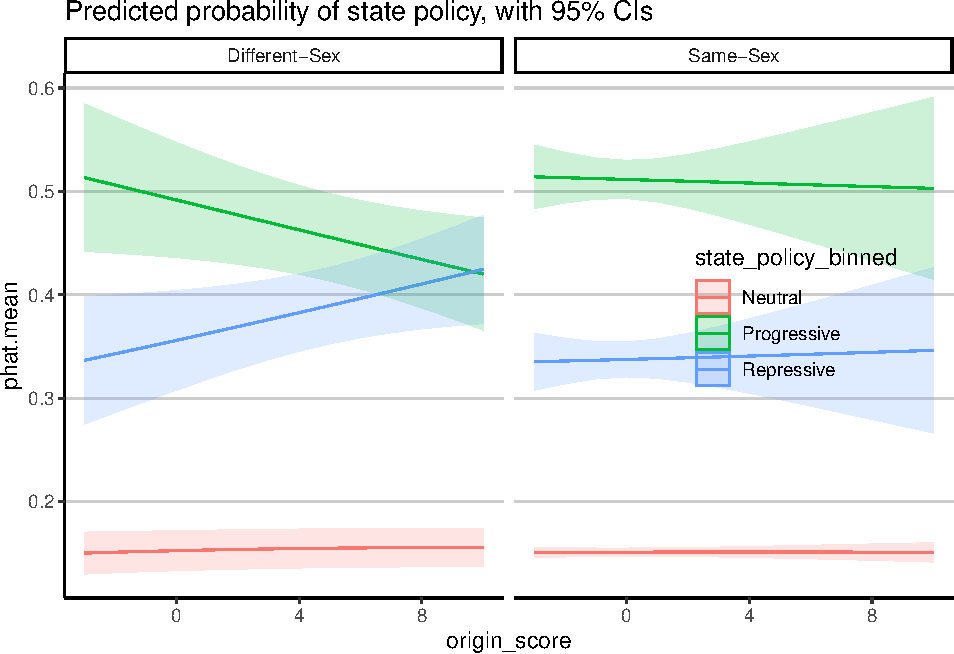
\includegraphics{ssimm_draft_files/figure-latex/sim-1.pdf}
\caption{\label{fig:sim}Predicted probabilities of U.S. state LGBT policy progressiveness for individual immigrants in different- and same-sex couples, based on policy score of sending country, with 95\% confidence intervals.}
\end{figure}

To help interpret these results, Figure \ref{fig:sim} contains predicted probabilities of residing in progressive, neutral, or repressive U.S. states. For each of 250 simulations, the coefficients are drawn from this covariance matrix as estimated in Model 3 in Table \ref{tab:ord}. These are used to predict the probably of being in each type of state for each member in the complete dataset, with their couple type set to same- or different-sex and their origin score varied from the minimum to maximum. The predicted probabilities are are averaged across the entire dataset for each of these manipulated values. After 250 simulations, the distribution of predicted values is used to find means and 95-percent confidence intervals. The only difference between the two panels is the value for the same-sex indicator in the simulations.

The figure shows opposite trends for same- and different-sex couples. Overall, immigrants tend to live in more progressive states, but the moderating effect of origin score is quite different for the two groups. The panel for same-sex couples shows that these immigrants tend to live in U.S. states with similar LGBT policy contexts to those of their countries of origin. Immigrants in same-sex couples from repressive countries are less likely to live in progressive U.S. states, but as the origin-country score increases, so does the probability of living in a progressive state. For immigrants in different-sex couples, on the other hand, increasingly progressive country-of-origin policies are associated with a \emph{lower} probability of residing in a progressive U.S. state, accompanied by a \emph{higher} probability of living in a repressive U.S. state. At the high end of the origin-score policy range, the difference in predicted probabilities is significant: typical immigrants in same-sex couples are percentage points more likely to live in progressive states and percentage points less likely to live in repressive states than similar immigrants in different-sex couples.

\hypertarget{sensitivity-analysis}{%
\subsection{Sensitivity Analysis}\label{sensitivity-analysis}}

We first assess how much our results would change in the presence of significant measurement error. \protect\hyperlink{ref-kreider_2015}{Kreider \& Lofquist} (\protect\hyperlink{ref-kreider_2015}{2015}) found that in the 2010 ACS, 57 percent of married and 7 percent of unmarried same-sex couples may have been different-sex couples that misreported a partner's sex. By 2016 the mismatch rate had declined to 31 percent of married and 3 percent of unmarried same-sex couples (\protect\hyperlink{ref-kreider_2017}{Kreider et al., 2017}).

Figure \ref{fig:sens} takes Model 3 form Table \ref{tab:country-props} and reduces the proportions of same-sex couples in the data. It varies the percentage of misreported same-sex married couples from 0 to 90 percent and of unmarried couples from 0 to 30 percent. Highlighted in blue bars are the empirical mismatch rates found in the two studies by Kreider et al. (\protect\hyperlink{ref-kreider_2017}{2017}; \protect\hyperlink{ref-kreider_2015}{2015}). We see that extremely high rates of misreporting are necessary to reduce this effect to 0.

We next text the robustness of our results to omitted variable bias.

\hypertarget{discussion}{%
\section{Discussion}\label{discussion}}

In 2013, there were 61 thousand same-sex couples that included immigrants in the U.S. By 2019, this number had nearly doubled to 107 thousand (\protect\hyperlink{ref-u.s.censusbureau_2020}{U.S. Census Bureau, 2020}). Despite this expansive growth of same-sex immigrant couples in the U.S. far outpacing overall migration rates, there is little demographic research understanding the characteristics of these couples or the factors influencing their migratory patterns. Consequently, we know little about who these migrants are, why they are choosing to leave their home countries, or where they are choosing to locate once in the U.S. Answering these questions is important, not just because this represents an increasing number of border crossers, but because this process has the potential to reshape our conceptualization of who immigrants are and their motivations for moving.

The rising number of same-sex immigrant couples has coincided with a dramatic change in policy environments governing LGBT communities -- both within the U.S. and abroad. Indeed, it is precisely because of this changing policy environment, namely around the 2013 DOMA Supreme Court case, that same-sex couples now have a legal pathway into the U.S. that does not rely on asylum claims. Therefore, although there are numerous perspectives to take in understanding the migratory patterns of these couples, this project specifically investigates how changing LGBT policies at both country of origin and residing U.S. state pattern these migratory pathways. Engaging in such a question adds to emerging scholarship trying to understand how dramatic policy changes are influencing the health, well-being, and lifestyles of LGBT people while also recognizing that these policies differentially impact people within this broad umbrella based on different social positions (xx). Moreover, it helps to address an important gap within migration studies that too often discount the role of the state and the salience of sexuality in conditioning migratory patterns (\protect\hyperlink{ref-carrillo_2018}{Carrillo, 2018}; \protect\hyperlink{ref-fitzgerald_2014}{Fitzgerald et al., 2014}).

To answer this question, we take advantage of an underutilized data source: self-reports of same-sex immigrant couples in the American Community Survey from 2008-2019. Despite this resource being one of the few national surveys to capture same-sex couples or immigrant couples, these data are virtually untapped for this purpose. Few studies use the ACS to analyze same-sex couples, and the ones that do largely focus on residential segregation (e.g. \protect\hyperlink{ref-poston_2017}{Poston et al., 2017}). Therefore, these data allow for us to make one of the first large-\(N\) investigations of same-sex immigrant couples within the U.S. and to make an important correction to this area of scholarship.

Using these data, we make a number of interesting findings worth detailing. First, existing scholarship on same-sex immigrant couples, and queer migration more broadly, largely focuses on the asylum and refugee processes. This is because this was one of the only mechanisms to get into the U.S. (\protect\hyperlink{ref-humanrightswatch_2006}{Human Rights Watch, 2006}); xx). Consequently, this over-representation distorts our understanding of who same-sex immigrant couples are, the types of environments they are leaving from, and their motivations to seek entry into the U.S. Indeed, when comparing the demographics of same-sex immigrant couples to different-sex immigrant couples, we find same-sex couples generally have higher incomes and occupational prestige and are somewhat more educated. Understanding this profile alone is an important insight as it reveals that these communities are of privileged social standing. This is a corrective to the queer migration literature that has yet to highlight this profile. It is interesting that, although it is known migration is a taxing endeavor, migrants in same-sex couples come from stronger social positions than migrants in different-sex relationships.

Understanding who these migrants are, how do LGBT policies in their countries of origin influence their desires to come to the U.S.? Despite existing scholarship portraying a story of LGB couples fleeing repression, as necessary for refugee claims, LGB couples are leaving countries with more progressive policy environments. As results in Table \ref{tab:country-props} and trendlines in Figure \ref{fig:policy-desc} reveal, couples are coming from more open environments. This is true even after accounting for more traditional gravity model variables that primarily focus on economic costs and benefits to migration. Though more research is needed, these results, in conjunction with the fact that these same-sex couples achieve higher incomes and greater occupational prestige, describe a situation in which perhaps it is the supportive policy environment, such as employment protections, access to the material benefits of marriage, and so forth, that enable same-sex couples to achieve greater social standing and the resources necessary to migrate. Or, instead of the immediate benefits of the policy itself, these supportive environments may simply encourage LGB people to feel comfortable to openly identify as being in a relationship when asked by surveyors.

One unexpected finding is different-sex couples from more LGBT-friendly countries are likelier to reside in states with increasingly less LGBT-friendly policies. These patterns in Figure \ref{fig:sim} are peculiar because we suspected that state LGBT policies to have no association with how different-sex couples are making decisions as to where to reside. This is not the case. One immediate question this raises is if this is a case of ``straight flight.'' White flight is a well-research process in which white people leave diversifying communities. After straight couples experience liberalized conditions for gay couples, do they intentionally seek to leave such conditions by moving to states that are less supportive? More research is needed to understand this pattern.

Recent research has argued that sexuality is a salient factor determining immigration decisions. We show that differences between immigrants in same-sex couples and those in different-sex couples cannot be explained solely using classic theories of migration; policy context and sexuality interact in complicated ways to shape migratory flows. This points to the importance of further studying the interaction between the state and identity in migratory processes.

\hypertarget{references}{%
\section{References}\label{references}}

\setlength{\parindent}{-0.2in}
\setlength{\leftskip}{0.2in}
\setlength{\parskip}{8pt}

\noindent

\hypertarget{refs}{}
\begin{CSLReferences}{1}{0}
\leavevmode\hypertarget{ref-adur_2018}{}%
Adur, S. M. (2018). In pursuit of love: {`{Safe} passages,'} migration and queer {South} {Asians} in the {US}. \emph{Current Sociology}, \emph{66}(2), 320--334.

\leavevmode\hypertarget{ref-anderson_2011}{}%
Anderson, J. E. (2011). The {Gravity} {Model}. \emph{Annual Review of Economics}, \emph{3}(1), 133--160. \url{https://doi.org/10.1146/annurev-economics-111809-125114}

\leavevmode\hypertarget{ref-ayoub_2016}{}%
Ayoub, P. (2016). \emph{When {States} {Come} {Out}}. Cambridge University Press.

\leavevmode\hypertarget{ref-ayoub_2017}{}%
Ayoub, P., \& Garretson, J. (2017). Getting the message out: {Media} context and global changes in attitudes toward homosexuality. \emph{Comparative Political Studies}, \emph{50}(8), 1055--1085.

\leavevmode\hypertarget{ref-baumle_2009}{}%
Baumle, A. K., Compton, D., \& Poston, D. L. (2009). \emph{Same-{Sex} {Partners}: {The} {Social} {Demography} of {Sexual} {Orientation}}. SUNY Press.

\leavevmode\hypertarget{ref-bea_2020}{}%
BEA. (2020). \emph{Regional {Data}: {GDP} and {Personal} {Income}}. Bureau of Economic Analysis, U.S. Department of Commerce. \url{https://apps.bea.gov/iTable/iTable.cfm?acrdn=1\&isuri=1\&reqid=70\&step=1\#reqid=70\&step=1\&isuri=1}

\leavevmode\hypertarget{ref-beaudin_2017}{}%
Beaudin, L. (2017). Marriage equality and interstate migration. \emph{Applied Economics}, \emph{49}(30), 2956--2973. \url{https://doi.org/10.1080/00036846.2016.1251565}

\leavevmode\hypertarget{ref-beine_2016}{}%
Beine, M., Bertoli, S., \& Moraga, J. F.-H. (2016). A {Practitioners}' {Guide} to {Gravity} {Models} of {International} {Migration}. \emph{The World Economy}, \emph{39}(4), 496--512. https://doi.org/\url{https://doi.org/10.1111/twec.12265}

\leavevmode\hypertarget{ref-benson_2012}{}%
Benson, M., \& O'Reilly, K. (2012). \emph{Lifestyle {Migration}: {Expectations}, {Aspirations} and {Experiences}} (Har/Ele edition). Ashgate.

\leavevmode\hypertarget{ref-bls_2020}{}%
BLS. (2020). \emph{Monthly state unemployment rates}. U.S. Bureau of Labor Statistics. \url{https://download.bls.gov/pub/time.series/la/la.data.3.AllStatesS}

\leavevmode\hypertarget{ref-boertien_2019}{}%
Boertien, D., \& Vignoli, D. (2019). Legalizing same-sex marriage matters for the subjective well-being of individuals in same-sex unions. \emph{Demography}, \emph{56}(6), 2109--2121.

\leavevmode\hypertarget{ref-canaday_2009}{}%
Canaday, M. (2009). \emph{The straight state: Sexuality and citizenship in twentieth-century {America}}. Princeton University Press.

\leavevmode\hypertarget{ref-cantu_2009}{}%
Cantú, L. (2009). \emph{The {Sexuality} of {Migration}: {Border} {Crossings} and {Mexican} {Immigrant} {Men}} (N. A. Naples \& S. Vidal-Ortiz, Eds.). NYU Press.

\leavevmode\hypertarget{ref-carpenter_2020}{}%
Carpenter, C. S. (2020). The {Direct} {Effects} of {Legal} {Same}-{Sex} {Marriage} in the {United} {States}: {Evidence} {From} {Massachusetts}. \emph{Demography}, \emph{57}(5), 1787--1808.

\leavevmode\hypertarget{ref-carrillo_2018}{}%
Carrillo, H. (2018). \emph{Pathways of {Desire}: {The} {Sexual} {Migration} of {Mexican} {Gay} {Men}}. University of Chicago Press.

\leavevmode\hypertarget{ref-corey-boulet_2019}{}%
Corey-Boulet, R. (2019). \emph{Love {Falls} on {Us}: A story of {American} ideas and {African} {LGBT} lives}. Zed Books Ltd.

\leavevmode\hypertarget{ref-epstein_2014}{}%
Epstein, S., \& Carrillo, H. (2014). Immigrant sexual citizenship: Intersectional templates among {Mexican} gay immigrants to the {USA}. \emph{Citizenship Studies}, \emph{18}(3-4), 259--276. \url{https://doi.org/10.1080/13621025.2014.905266}

\leavevmode\hypertarget{ref-feenstra_2015}{}%
Feenstra, R. C., Inklaar, R., \& Timmer, M. P. (2015). The {Next} {Generation} of the {Penn} {World} {Table}. \emph{American Economic Review}, \emph{105}(10), 3150--3182. \url{https://doi.org/10.1257/aer.20130954}

\leavevmode\hypertarget{ref-feliciano_2020}{}%
Feliciano, C. (2020). Immigrant {Selectivity} {Effects} on {Health}, {Labor} {Market}, and {Educational} {Outcomes}. \emph{Annual Review of Sociology}, \emph{46}(1), 315--334. \url{https://doi.org/10.1146/annurev-soc-121919-054639}

\leavevmode\hypertarget{ref-fisher_2018}{}%
Fisher, R., Gee, G., \& Looney, A. (2018). Same-{Sex} {Married} {Tax} {Filers} {After} {Windsor} and {Obergefell}. \emph{Demography}, \emph{55}(4), 1423--1446. \url{https://doi.org/10.1007/s13524-018-0684-5}

\leavevmode\hypertarget{ref-fitzgerald_2014}{}%
Fitzgerald, J., Leblang, D., \& Teets, J. C. (2014). Defying the {Law} of {Gravity}: {The} {Political} {Economy} of {International} {Migration}. \emph{World Politics}, \emph{66}(3), 406--445. \url{https://doi.org/10.1017/S0043887114000112}

\leavevmode\hypertarget{ref-gates_2013}{}%
Gates, G. J. (2013a). \emph{{LGBT} {Adult} {Immigrants} in the {United} {States}}. The Williams Institute. \url{https://escholarship.org/uc/item/2cj0k29c}

\leavevmode\hypertarget{ref-gates_2009a}{}%
Gates, G. J. (2009). \emph{{FAQ}: {Same}-{Sex} {Couples} in the 2008 {American} {Community} {Survey}}. The Williams Institute. \url{https://escholarship.org/uc/item/5rm9m88p}

\leavevmode\hypertarget{ref-gates_2013a}{}%
Gates, G. J. (2013b). Geography of the {LGBT} population. In \emph{International handbook on the demography of sexuality} (pp. 229--242). Springer.

\leavevmode\hypertarget{ref-giametta_2020}{}%
Giametta, C. (2020). New asylum protection categories and elusive filtering devices: The case of {`{Queer} asylum'} in {France} and the {UK}. \emph{Journal of Ethnic and Migration Studies}, \emph{46}(1), 142--157.

\leavevmode\hypertarget{ref-giddings_2014}{}%
Giddings, L., Nunley, J. M., Schneebaum, A., \& Zietz, J. (2014). Birth {Cohort} and the {Specialization} {Gap} {Between} {Same}-{Sex} and {Different}-{Sex} {Couples}. \emph{Demography}, \emph{51}(2), 509--534. \url{https://doi.org/10.1007/s13524-013-0267-4}

\leavevmode\hypertarget{ref-goldberg_2021}{}%
Goldberg, S. K., \& Conron, K. J. (2021). \emph{{LGBT} {Adult} {Immigrants} in the {United} {States}}. The Williams Institute. \url{https://escholarship.org/uc/item/2cj0k29c}

\leavevmode\hypertarget{ref-gonzalez-lopez_2005}{}%
González-López, G. (2005). \emph{Erotic {Journeys}}. University of California Press.

\leavevmode\hypertarget{ref-goodnature_2021}{}%
Goodnature, M., \& Neto, A. B. F. (2021). Same-{Sex} {Unmarried} {Partners} in the {Census}. \emph{Journal of Regional Analysis \& Policy}, \emph{51}(1), 43--66. \url{https://jrap.scholasticahq.com/article/22080-same-sex-unmarried-partners-in-the-census}

\leavevmode\hypertarget{ref-hatton_2005a}{}%
Hatton, T. J., \& Williamson, J. G. (2005). \emph{Global {Migration} and the {World} {Economy}: {Two} {Centuries} of {Policy} and {Performance}}. The MIT Press. \url{https://doi.org/10.7551/mitpress/3303.001.0001}

\leavevmode\hypertarget{ref-hondagneu-sotelo_2012}{}%
Hondagneu-Sotelo, P. (2012). New directions in gender and immigration research. In \emph{Routledge {International} {Handbook} of {Migration} {Studies}}. Routledge. \url{https://doi.org/10.4324/9780203863299.ch15}

\leavevmode\hypertarget{ref-humanrightswatch_2006}{}%
Human Rights Watch. (2006). \emph{Family, {Unvalued}: {Discrimination}, {Denial}, and the {Fate} of {Binational} {Same}-{Sex} {Couples} under {U}.{S}. {Law}}. \url{https://www.hrw.org/sites/default/files/reports/FamilyUnvalued.pdf}

\leavevmode\hypertarget{ref-joyner_2017}{}%
Joyner, K., Manning, W., \& Bogle, R. (2017). Gender and the {Stability} of {Same}-{Sex} and {Different}-{Sex} {Relationships} {Among} {Young} {Adults}. \emph{Demography}, \emph{54}(6), 2351--2374. \url{https://doi.org/10.1007/s13524-017-0633-8}

\leavevmode\hypertarget{ref-kail_2015}{}%
Kail, B. L., Acosta, K. L., \& Wright, E. (2015). State-level marriage equality and the health of same-sex couples. \emph{American Journal of Public Health}, \emph{105}(6), 1101--1105.

\leavevmode\hypertarget{ref-karemera_2000}{}%
Karemera, D., Oguledo, V. I., \& Davis, B. (2000). A gravity model analysis of international migration to {North} {America}. \emph{Applied Economics}, \emph{32}(13), 1745--1755. \url{https://doi.org/10.1080/000368400421093}

\leavevmode\hypertarget{ref-karimi_2020}{}%
Karimi, A. (2020). Refugees' {Transnational} {Practices}: {Gay} {Iranian} {Men} {Navigating} {Refugee} {Status} and {Cross}-border {Ties} in {Canada}. \emph{Social Currents}, \emph{7}(1), 71--86.

\leavevmode\hypertarget{ref-kazyak_2018}{}%
Kazyak, E., Burke, K., \& Strange, M. (2018). Logics of {Freedom}: {Debating} {Religious} {Freedom} {Laws} and {Gay} and {Lesbian} {Rights}. \emph{Socius}, \emph{4}, 1--18.

\leavevmode\hypertarget{ref-klawitter_2015}{}%
Klawitter, M. (2015). Meta-{Analysis} of the {Effects} of {Sexual} {Orientation} on {Earnings}. \emph{Industrial Relations: A Journal of Economy and Society}, \emph{54}(1), 4--32. \url{https://doi.org/10.1111/irel.12075}

\leavevmode\hypertarget{ref-kreider_2017}{}%
Kreider, R. M., Bates, N., \& Mayol-García, Y. (2017). Improving measurement of same-sex couple households in {Census} {Bureau} surveys: {Results} from recent tests. \emph{{PAA} 2017 Annual Meeting}.

\leavevmode\hypertarget{ref-kreider_2015}{}%
Kreider, R. M., \& Lofquist, D. A. (2015). Matching survey data with administrative records to evaluate reports of same-sex married couple households. \emph{Washington, DC: US Census Bureau}.

\leavevmode\hypertarget{ref-lax_2009}{}%
Lax, J. R., \& Phillips, J. H. (2009). Gay rights in the states: {Public} opinion and policy responsiveness. \emph{American Political Science Review}, \emph{103}(3), 367--386.

\leavevmode\hypertarget{ref-levy_2017}{}%
Levy, B. L., \& Levy, D. L. (2017). When {Love} {Meets} {Hate}: {The} {Relationship} {Between} {State} {Policies} on {Gay} and {Lesbian} {Rights} and {Hate} {Crime} {Incidence}. \emph{Social Science Research}, \emph{61}, 142--159.

\leavevmode\hypertarget{ref-luibheid_2008}{}%
Luibhéid, E. (2008). Queer/{Migration}: {An} {Unruly} {Body} of {Scholarship}. \emph{GLQ: A Journal of Lesbian and Gay Studies}, \emph{14}(2-3), 169--190. \url{https://doi.org/10.1215/10642684-2007-029}

\leavevmode\hypertarget{ref-luibheid_2005}{}%
Luibhéid, E., \& Cantú, L. (2005). \emph{Queer {Migrations}: {Sexuality}, {U}.{S}. {Citizenship}, and {Border} {Crossings}}. U of Minnesota Press.

\leavevmode\hypertarget{ref-lutz_2010}{}%
Lutz, H. (2010). Gender in the {Migratory} {Process}. \emph{Journal of Ethnic and Migration Studies}, \emph{36}(10), 1647--1663. \url{https://doi.org/10.1080/1369183X.2010.489373}

\leavevmode\hypertarget{ref-manning_2016}{}%
Manning, W. D., Brown, S. L., \& Stykes, J. B. (2016). Same-{Sex} and {Different}-{Sex} {Cohabiting} {Couple} {Relationship} {Stability}. \emph{Demography}, \emph{53}(4), 937--953. \url{https://doi.org/10.1007/s13524-016-0490-x}

\leavevmode\hypertarget{ref-marshall_2018}{}%
Marshall, M. G. (2018). \emph{Polity5: {Dataset} {Users}' {Manual}}. Center for Systemic Peace; Societal-Systems Research Inc.

\leavevmode\hypertarget{ref-massey_1987}{}%
Massey, D. S., Alarcon, R., Durand, J., \& González, H. (1987). \emph{Return to {Aztlan}: {The} {Social} {Process} of {International} {Migration} from {Western} {Mexico}}. University of California Press.

\leavevmode\hypertarget{ref-massey_1999}{}%
Massey, D. S., Arango, J., Hugo, G., Kouaouci, A., Pellegrino, A., \& Taylor, J. E. (1999). \emph{Worlds in {Motion}: {Understanding} {International} {Migration} at the {End} of the {Millennium}}. Oxford University Press.

\leavevmode\hypertarget{ref-mayda_2010}{}%
Mayda, A. M. (2010). International migration: A panel data analysis of the determinants of bilateral flows. \emph{Journal of Population Economics}, \emph{23}(4), 1249--1274. \url{https://www.jstor.org/stable/40925859}

\leavevmode\hypertarget{ref-mayer_2011}{}%
Mayer, T., \& Zignago, S. (2011). Notes on {CEPII}'s {Distances} {Measures}: {The} {GeoDist} {Database}. \emph{SSRN Electronic Journal}. \url{https://doi.org/10.2139/ssrn.1994531}

\leavevmode\hypertarget{ref-michaels_2013}{}%
Michaels, S. (2013). Sexual behavior and practices: {Data} and measurement. In \emph{International handbook on the demography of sexuality} (pp. 11--20). Springer.

\leavevmode\hypertarget{ref-mole_2018a}{}%
Mole, R. (2018). Sexualities and queer migration research. \emph{Sexualities}, \emph{21}(8), 1268--1270.

\leavevmode\hypertarget{ref-murray_2016}{}%
Murray, D. A. B. (2016). \emph{Queering {Borders}: {Language}, {Sexuality}, and {Migration}}. John Benjamins Publishing Company.

\leavevmode\hypertarget{ref-ozden_2011}{}%
Özden, Ç., Parsons, C. R., Schiff, M., \& Walmsley, T. L. (2011). Where on {Earth} is {Everybody}? {The} {Evolution} of {Global} {Bilateral} {Migration} 1960--2000. \emph{The World Bank Economic Review}, \emph{25}(1), 12--56. \url{https://doi.org/10.1093/wber/lhr024}

\leavevmode\hypertarget{ref-palloni_2001}{}%
Palloni, A., Massey, D. S., Ceballos, M., Espinosa, K., \& Spittel, M. (2001). Social {Capital} and {International} {Migration}: {A} {Test} {Using} {Information} on {Family} {Networks}. \emph{American Journal of Sociology}, \emph{106}(5), 1262--1298. \url{https://doi.org/10.1086/320817}

\leavevmode\hypertarget{ref-poot_2016}{}%
Poot, J., Alimi, O., Cameron, M. P., \& Maré, D. C. (2016). \emph{The {Gravity} {Model} of {Migration}: {The} {Successful} {Comeback} of an {Ageing} {Superstar} in {Regional} {Science}} (SSRN Scholarly Paper ID 2864830). Social Science Research Network. \url{https://papers.ssrn.com/abstract=2864830}

\leavevmode\hypertarget{ref-portes_1998}{}%
Portes, A. (1998). Social {Capital}: {Its} {Origins} and {Applications} in {Modern} {Sociology}. \emph{Annual Review of Sociology}, \emph{24}(1), 1--24. \url{https://doi.org/10.1146/annurev.soc.24.1.1}

\leavevmode\hypertarget{ref-poston_2017}{}%
Poston, D. L. J., Compton, D. R., Xiong, Q., \& Knox, E. A. (2017). The {Residential} {Segregation} of {Same}-{Sex} {Households} from {Different}-{Sex} {Households} in {Metropolitan} {USA}, circa-2010. \emph{Population Review}, \emph{56}(2). \url{https://doi.org/10.1353/prv.2017.0005}

\leavevmode\hypertarget{ref-ruggles_2021}{}%
Ruggles, S., Flood, S., Foster, S., Goeken, R., Pacas, J., Schouweiler, M., \& Sobek, M. (2021). \emph{{IPUMS} {USA}: {Version} 11.0 {American} {Community} {Survey} 2008-2019.} IPUMS. \url{https://doi.org/10.18128/D010.V11.0}

\leavevmode\hypertarget{ref-schwartz_2009}{}%
Schwartz, C., \& Graf, N. (2009). Assortative matching among same-sex and different-sex couples in the {United} {States}, 1990-2000. \emph{Demographic Research}, \emph{21}(28), 843--878. \url{https://doi.org/10.4054/DemRes.2009.21.28}

\leavevmode\hypertarget{ref-soule_2004}{}%
Soule, S. (2004). Going to the chapel? {Same}-sex marriage bans in the {United} {States}, 1973--2000. \emph{Social Problems}, \emph{51}(4), 453--477.

\leavevmode\hypertarget{ref-stella_2020}{}%
Stella, F., \& Gawlewicz, A. (2020). Social networks, language and identity negotiations among queer migrants in {Scotland}. \emph{Journal of Ethnic and Migration Studies}, 1--19.

\leavevmode\hypertarget{ref-todaro_1980}{}%
Todaro, M. (1980). Internal migration in developing countries: A survey. In \emph{Population and economic change in developing countries} (pp. 361--402). University of Chicago Press.

\leavevmode\hypertarget{ref-u.s.censusbureau_2013}{}%
U.S. Census Bureau. (2013). \emph{Frequently {Asked} {Questions} {About} {Same}-{Sex} {Couple} {Households}}. U.S. Census Bureau Fertility; Family Statistics Branch.

\leavevmode\hypertarget{ref-u.s.censusbureau_2017}{}%
U.S. Census Bureau. (2017). \emph{American {Community} {Survey} {Information} {Guide}}. U.S. Census Bureau. \url{https://www.census.gov/programs-surveys/acs/about/information-guide.html}

\leavevmode\hypertarget{ref-u.s.censusbureau_2020}{}%
U.S. Census Bureau. (2020). \emph{2008-2019 {American} {Community} {Survey} {Public} {Use} {Microdata} {Samples}}. \url{https://usa.ipums.org/usa/index.shtml}

\leavevmode\hypertarget{ref-unhcr_2008}{}%
UNHCR. (2008). \emph{Claims to {Refugee} {Status} based on {Sexual} {Orientation} and/or {Gender} {Identity} within the context of {Article} {1A}(2) of the 1951 {Convention} and/or its 1967 {Protocol} relating to the {Status} of {Refugees}}. United Nations High Commissioner for Refugees. \url{https://www.unhcr.org/509136ca9.pdf}

\leavevmode\hypertarget{ref-unitednations_2017}{}%
United Nations. (2017). \emph{Trends in {International} {Migrant} {Stock}: {The} 2017 {Revision} ({United} {Nations} database, {POP}/{DB}/{MIG}/{Stock}/{Rev}.2017)}. Suggested citation: United Nations, Department of Economic; Social Affairs, Population Division. \url{https://www.un.org/en/development/desa/population/migration/data/estimates2/estimates17.asp}

\leavevmode\hypertarget{ref-velasco_2020}{}%
Velasco, K. (2020). A {Growing} {Queer} {Divide}: {The} {Divergence} between {Transnational} {Advocacy} {Networks} and {Foreign} {Aid} in {Diffusing} {LGBT} {Policies}. \emph{International Studies Quarterly}, \emph{64}(1), 120--132. \url{https://doi.org/10.1093/isq/sqz075}

\leavevmode\hypertarget{ref-velasco_2018}{}%
Velasco, K. (2018). Human {Rights} {INGOs}, {LGBT} {INGOs}, and {LGBT} {Policy} {Diffusion}, 1991--2015. \emph{Social Forces}, \emph{97}(1), 377--404. \url{https://doi.org/10.1093/sf/soy030}

\leavevmode\hypertarget{ref-vogler_2016}{}%
Vogler, S. (2016). Legally {Queer}: {The} {Construction} of {Sexuality} in {LGBQ} {Asylum} {Claims}. \emph{Law \& Society Review}, \emph{50}(4), 856--889. \url{https://doi.org/10.1111/lasr.12239}

\leavevmode\hypertarget{ref-worldbank_2020}{}%
World Bank. (2020). \emph{Unemployment, total (\% of total labor force) (modeled {ILO} estimate)}. International Labour Organization, ILOSTAT database. \url{https://data.worldbank.org/indicator/SL.UEM.TOTL.ZS}

\end{CSLReferences}

\end{document}
